\documentclass[a4paper,12pt,oneside,openright]{article}
\usepackage[pdftex] {graphicx}
\usepackage[utf8]{inputenc}
\usepackage{listings}
\usepackage{graphicx}
\usepackage{subfig}
\usepackage{chapterbib}

\usepackage{algorithm}
\usepackage{algorithmic}
\usepackage{wrapfig}

\addtolength{\hoffset}{-1cm}
\addtolength{\textwidth}{2.5cm}

\lstdefinelanguage{J}[]{C}
{morekeywords={},
sensitive=false}
\lstset{language=J}
% shadowbox come frame
% rulesepcolor=\color{Gray}
\lstset{frame=trBL}
\lstset{frameround=fttt}
\lstset{tabsize=3, breaklines, commentstyle=\texttt}
\lstset{showstringspaces=false}
\lstset{basicstyle=\small}
\lstset{emph={},emphstyle=\textit}

\title{Performance evaluation of parallel sorting algorithms on large data sets - v0.9}
\author{Nicola Desogus, Paolo Giangrandi, Fabio Luporini}

\begin{document}
\maketitle
\tableofcontents
\pagebreak

\section{Introduction}
This project has the aim of studying the well known problem of sorting \textit{atomic} items (i.e. they occupy O(1) space) within the context of parallel computing. All the standard sequential sorting algorithms can be re-designed to exploit parallel machines; as a matter of fact, literature is not poor of this kind of works. There are some sequential algorithms (such as mergesort or quicksort) that can be easily adapted to the new parallel context; nevertheless, other ones needs a trickier re-engineering. On the other hand, algorithms that performs very well on sequential machines could not be so good in their new parallel version. Thus, the first objective of this project is to sperimentally compare the performance of the most known parallel sorting algorithms. 

In this scenario things get even more complicated from the fact that we have to manage very large data sets, i.e. our parallel algorithms sort terabytes of data. This means that some of the theoretical results achieved in the field of \textit{external memory sorting} will have to be compared with the ones that we will sperimentally obtain. Further, in order to keep implementation complexity limitated, we decide to not extends our algorithms for exploiting the presence of multi-disks eventually provided by the parallel architecture. 

In this complicated context the role of the test environment becomes crucial. Obvioulsy, we can not say neither that our algorithms will scale the same way on every possible parallel machine nor that results are meaningful only for a specifc machine. Hence, analyzing the results, we will have to consider even some fundamental architectural aspects. At a first glance, we have to take care of at least two macroscopic aspects: first, the possibility that the parallel machine is a hierarchycal systems (e.g. a cluster of shared memory nodes); second, the interconnection network of the nodes. In case of a hierarchycal system, if we will be able to find a way for exploiting the presence of shared memory, then we might achieve a very significative gain in terms of performance. Hence, depending both on the way we will exploit shared memory and the properties of the interconnection structure (bandwith, latency), we might get performance results more or less close to the ones we expected.

We will address all this issues both from a theoretical point of view and by implementing a structured framework. This document is organized as follows: first, we briefly explain which algorithms will be parallelized; second, we describe all the characteristcs of our framework; then, after having described the test environment, we will detail the implementation of our algorithms and, for each of them, we will analyze their performance. Finally, we will compare all the achieved results.

\section{Objectives, assumptions and algorithms}
\label{assumptions}
In the first part of our work we put a lot of efforts in deeply understanding the state of the art of parallel sorting algorithms. The first thing we noticed is the lack of an unified theory that asserts whether an algorithm is better than another; this is an obvious consequence of the absence of realistic cost models for parallel algorithms and architectures (e.g. both $PRAM$ and the more refined $LogP$ are too superficials to be considered significant. Second thing, the literature is rich of parallel algorithms conceived and engineered for \textit{specific machines}, so to be able to exploit peculiar features of the machine itself, e.g. the structure of the interconnection network. Just as examples we can cite~\cite{CSPA, CSPA2}, but with some googling we can really find a lot of papers or report on these themes. This approach is not obviously good because of at least two facts: the high designing complexity and the non-portability. Hence, in our project, even if the practical performance analysis will be done on a specific architecture, the parallel algorithms will \textit{not} be designed for that specific machine. In some sense, our approach is more close to~\cite{NPSA}.

We list the sorting algorithms that we are going to parallelize, all of them based on the Divide$\&$Conquer paradigm. Notice that, in general, the parallelization consist of ''exporting'' either the divide or the conquer phase to the ''process level''. Just as an example, in parallel Mergesort the distribution phase will be made between the processes of the parallel algorithm. 
\begin{enumerate}
\item Mergesort
\item K-Way Mergesort
\item Load-Balance Mergesort (and some variants) 
\item Quicksort
\item Bitonicsort
\item Bucketsort
\item Samplesort
\end{enumerate}
Examples of parallelization of $some$ of these algorithms can be find in literature. For instance, it is easy to find parallel versions of Mergesort, Quicksort, Samplesort, Bitonicsort. On the other hand, we notice the lack (or at least the poor availability) of informations regarding K-Way Mergesort and Load-Balance Mergesort. In any case, as we will better explain later, we re-implemented all the algorithms. Indeed, all the MPI implementations we found were really poor in terms of quality of code and do not take into account the possibility of having to sort large data sets, a problem which requires a specific analysis. Once implemented, we will compare the performance of these algorithms in terms of their efficiency, scalability and completion time, by playing on some degrees of freedom like the parallelism degree and the size of the data sets.  
 
In this section we will summarize the assumptions for this project, emerged during the several meetings.
\begin{itemize}
	\item{The work we need to do is to compare parallel sorting algorithms and to study how they behave. We early understood that to achieve such goal we were forced to collaborate in some way. We had to define a common framework in order to have comparable results. If any of us computed times in different ways, these wouldn't have been comparable. If any of us used a different strategy to sort data sequentially, or different optimization to sort data in principal memory or in disk, results would have been worthless, since the comparison would have mixed the performance of a parallel sorting algorithm with the performance of something else that regards sequential computation. This, besides, allowed us to do a better work, having a well structured framework which can be extended to many other algorithms with little work.}
	\item{We are not interested to study how sequential algorithms behave. We care only about the parallel part of our algorithms. The sequential part is always implemented using the \textit{qsort} POSIX standard function, and it does not matter if it works on primary memory only, rather than on secondary one. Sequential and parallel sorting are completely disjoint operations, which can be studied separately.}
	\item{Some algorithms natively begin, or end, with data centralized in a single process, while others begin or end with data distributed among all processes. For example mergesort begins with data distributed: any process sorts its piece fo data, and send it to another node that takes care of merging it, in order to end with data centralized on a single process. Quicksort, at the opposite, start with centralized data; the first process splits data and sends it to the other, in order to end up with distributed sorted data. For this reason and to mantain some homogenity among the algorithms we chose to always begin and end with centralized data. The algorithms that begin or end with distributed data will take care of scattering or gathering data, studying these extra (ie: unneeded by the algorithm, but needed by our common algorithm-testbed) operations separately from the rest of the computation.}
	\item{Since our platform is a clusted made of multicore nodes, we know that communication patterns between our several processes may weight a lot on the final performances. We will be looking for heuristical approaches to map processes in order to study what scenario will result in best performances due to communications between cores on different nodes, or on different parts of the single node.}
\end{itemize}


\section{Structuring the project: a top-down approach}
\subsection{Abstraction Layers}
As we have already said, we had to design a framework in such a way that our algorithms can share and exploit specific functionalities. In this context, it becomes useful to give a general view of the whole system by identifying and defining its abstraction layers, as shown in Figure~\ref{levels}. Let's briefly comment each of this levels and then focus on their specific features.
\begin{figure}[h]
  \begin{center}
    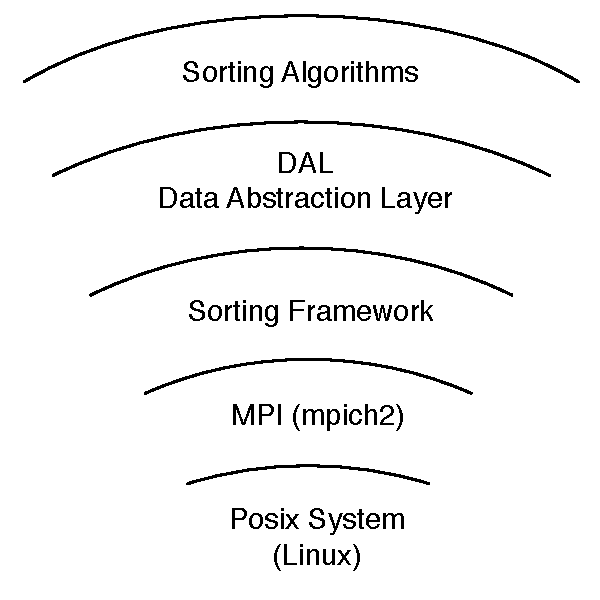
\includegraphics[scale=0.60]{levels}
  \end{center} 
  \caption{Abstract model}
  \label{levels}
\end{figure}
\begin{enumerate}
\item \textit{Sorting Algorithms.} The logic of a parallel sorting algorithm is defined at this level. The programmer works on primitives and data types provided by the DAL. It should be obvious, but we want to stress the fact that no visibility of MPI is provided at this level, that is the processes of a parallel algorithm communicate each other thanks to the communication primitives provided by the DAL.  
\item \textit{Data Abstraction Layer.} The DAL, as it will be better explained in~\ref{DAL}, allows us to decouple the designing of parallel algorithms from the necessity of handling data sets that can not fit the memory. 
\item \textit{Sorting Framework.} At this level we implemented a set of functionalities that are commons and essentials to every sorting algorithm: generation of datas, loading of data sets and storing of results, timing are the most important. 
\item \textit{MPI.} We used mpich2 because it allow us to place a specific process onto a specific core. TODO.
\item \textit{Posix System (Linux).} Almost all the upper levels exploit Posix mechanisms, e.g. for gathering times, argument parsing, dynamic loading. This is quite important because Linux becomes the only platform on which is possible to run the application (cygwin remains a secondary option). 
\end{enumerate}
In some sense, we can say that starting from a tool for parallel programming like MPI, we designed a new tool, namely the run-time support of the Sorting Algorithm level, that addresses our needs for implementing parallel sorting algorithm for large data sets. 

In the following we are going to describe each of these levels starting from the top-most one, namely Sorting Algorithms. The emphasis will be obvioulsy put on the firsts layers (Sorting Algorithms, DAL, Sorting Framework) which mainly represent the work we made in this project.


\subsection{Sorting Algorithms}
\subsection*{Terminology}
We briefly describe the terminology that we are going to use in this chapter. Our parallel algorithms have been implemented on top of MPI, thus they are composed by a set of $N$ processes, each of them having its unique identifier. According to the MPI terminology, we refer to a specific process by calling it $rank$ $x$, where $x \in N$ represents its identifier. The input sequence $S$ that has to be ordered is of size $n$. 

In order to define the \textit{efficiency} $\varphi$ of an algorithm, we have to introduce some parameters:
\begin{itemize}
\item $P$, the number of real processors of our machine; 
\item $m$, the number of steps of the algorithm;
\item $T_i$, the duration of step $i$ (in seconds);
\item $X_i$, a random variable which counts the number of real processors that contribute to the calculation during the step $i$.
\end{itemize}
Therefore, we can define the efficiency as:
\begin{center}
$\varphi = \frac{\sum_{i=0}^m \frac{E[X_i]}{P}}{m} = \frac{\sum_{i=0}^m E[X_i]}{P \times m} $
\end{center}
The efficiency is a formal tool to establish how much an algorithm exploits the parallelism degree of a machine. $\varphi \rightarrow 1$ means that the algorithm, in each step, tends to use all the available processor of the machine. Obviously, $\varphi \rightarrow 1$ does not means that the algorithm is ''good''; indeed, for such claim, the value of both $m$ and $T_i$ must be considered. For instance, we might have $\varphi \rightarrow 1$ and $T_i \rightarrow\infty$, meaning that each step requires a lot of time; or even worse, $m \rightarrow\infty$, meaning that the algorithm requires a lot of steps in which almost all the processors are involved.

As we said, a parallel sorting algorithm is composed of some steps of computation. During each step, a process can do basically three things, obviouslly not mutual exclusive each other:
\begin{itemize}
\item it can send data to other processes (the process is a \textit{sender} of that step)
\item it can receive data from other processes (the process is a \textit{receiver} of that step)
\item it can perform computation.
\end{itemize}

\subsection{Mergesort}
Mergesort is a well-known sorting algorithm based on the Divide$\&$Conquer paradigm. Thinking to a parallel version of Mergesort is therefore quite natural. First of all, $S$ is scattered among the $N$ processes. Each process locally sorts its own portion of $\frac{n}{N}$ elements, using a standard sequential sorting algorithm, like \textit{qsort}. At this point, a sequence of $\lceil \log_{2}{N} \rceil$ steps starts; in everyone of them, a \textit{distribution} phase precedes a \textit{merging} phase. The distribution phase is performed \textit{between different processes}: for instance, $rank$ $1$ sends its data to $rank$ $0$, while $rank$ $3$ to $rank$ $2$ and so on. On the other hand, the merging phase is done locally by all the processes that received a portion of datas. Figure~\ref{merge-dist} clarifies these concepts. Further, we observe that as its sequential counterpart, our version of mergesort needs an auxiliary array of size $n$. 
\begin{algorithmic}[1]  
	\medskip
	\STATE $Scatter( S, S\_local )$
	\STATE $qsort( S\_local )$
	\REPEAT 
		\STATE $distribution( S\_local )$
		\STATE $fusion ( S\_local )$
	\UNTIL $i < \log_{2}{N}$
	\medskip
\label{alg1}
\end{algorithmic}
Notice that steps $\lbrace 1, 2 \rbrace$ will be tipically perfermed by all our algorithms, not just by Mergesort. We conclude this overview by emphasizing that the \textit{distribution} of datas in each step can be handled in many different ways; that is, there are many possibile communication patterns between processes, that may lead to different performance behaviour (for instance, because of the change of the load on the interconnection structure) . We will address this important topic in a following section.

\begin{figure}[h]
        \centerline{
               \mbox{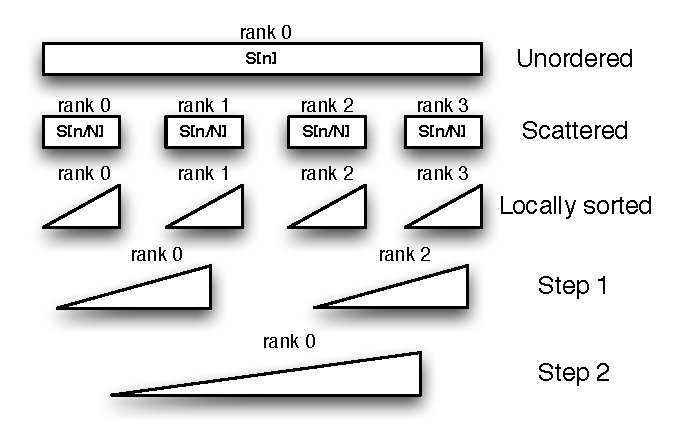
\includegraphics[scale=0.70]{mergesort-pict1}}
        }
        \caption{Parallel mergesort for $N = 4$.}
        \label{merge-dist}
\end{figure}

\subsubsection*{Parallel version}
\subsubsection*{Mapping virtual processors onto different cores} 
\subsubsection*{Performance Analisys} 
\subsubsection*{Efficiency} 
\subsubsection*{statistical analysys}

%\subsubsection{Parallel version}
%Descrizione della parallelizzazione dell'algoritmo; possibile uso di pseudocodice. Per lo pseudocodice ho definito in Relazione.tex un template da poter utilizzare. Ad esempio, se voglio includere lo pseudocodice del mergesore, basta scrivere: $lstinputlisting{mergesort.code}$. Per convenzione i file con lo pseudocodice scriviamoli con estensione .code.
%\subsubsection{Mapping virtual processors onto different cores} 
%only if they are considered in the specific version
%\subsubsection{Performance Analisys} 
%Qua discutiamo di completion time e quindi scalability ecc. Magari facciamo un confronto con quelle che devono essere le prestazioni ideali.
%\subsubsection{Efficiency} 
%Magari il nome di questa sezione va ''raffinato''..cmq, qua discutiamo di quello che diceva il coppola, cioè ad ogni step dell'ordinamento quanto riusciamo a sfruttare l'architettura parallela. Magari c soffermiamo su quanto la presenza del multicore sia effettivamente sfruttata e quanto. 
%\subsubsection{statistical analysys}
%to be discussed in case variance is high...questo magari possiamo scriverlo DOPO aver fatto i test.

\subsubsection{K-Way Mergesort}
\label{kmerge}
The idea of sequential K-Way Mergesort is to enhance the merging phase by enlarging to $K$ the number of runs that are fused at a time. This approach, designed in the context of external-memory model, aims at reducing the I/O-complexity of Mergesort by improving the memory space utilization~\cite{FERR}. 

We reuse this idea, but with different purposes, to get another parallel version of Mergesort: now, the objective is not to lower the I/O-complexity, but rather to improve the \textit{efficiency}, that is both to diminish the number of steps of the algorithm and to increase the number or computing processor at each step. An initialization phase takes place as in Mergesort: $S$ is scattered among the processes and it is locally sorted. With respect to Mergesort, the distribution phase needs to be modified. While in Mergesort, in each step, there were exactly many senders as many receivers ($\frac{\sharp senders}{\sharp receivers} = 1$), in K-Way Mergesort the number of senders is higher ( $\frac{\sharp senders}{\sharp receivers} = K - 1$, see figure~\ref{k-merge-dist}). In other words, in a specific step, a process may receive data from $K-1$ processes. This approach allows us to reduce $m$ with respect to Mergesort. The merging phase is performed locally by the processes that have received $K-1$ blocks of data during the step. From sequential K-Way Mergesort we know that the best way to implement the fusion of more than two runs is to use a Heap data structure~\cite{FERR}; since in our parallel context the merging phase is not modified, we re-adopt the same approach.

We notice that in K-Way Mergesort the average value of $T_i$ may be different from the one we obtained for Mergesort. This is may due both to a longer merging phase and to the potential conflicts that may arise on the interconnection structure when $K-1$ processes try to send data to the same specific process.

\begin{figure}[h]
        \centerline{
               \mbox{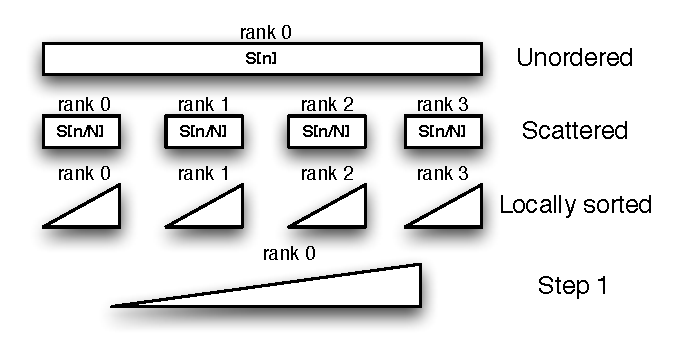
\includegraphics[scale=0.70]{kmerge-pict1}}
        }
        \caption{Parallel mergesort for $N = 4$, $K = 4$.}
        \label{k-merge-dist}
\end{figure}

\subsubsection*{Mapping virtual processors onto different cores} 

\subsubsection{Load-Balanced Merge Sort}
When we refer to load balancing, we ideally want all the processes to be operating continuously in the overall computation, which would lead to the minimum execution time. Achieving this goal by spreading the work evenly across processes is called load balancing.

The main limit of the classic approach in parallelizing merge sort is due to the number of idle processes that keeps growing during the merging phase. The active processes are halved at each step. Therefore, the maximum achievable efficiency is severely limited. The aim of the \textit{Load-Balanced Merge Sort} we implemented is to force each process to participate in the entire merging phase in order to obtain higher parallelism and increase efficiency.

To define the range of numbers on which a process will operate during the merge, a preprocessing phase is required. A regular sampling scheme is exploited to picks out $n-1$ numbers, $s_1$, $s_2$, \dots, $s_{n-1}$, from the input sequence $S$ as \textit{splitters}. At the end of the overall computation, the partition of process $i$ will contain elements $e$ for which $s_{i-1} \leq e < s_i$.

At this point, a loop of $\log (n)$ steps starts. At each step $i$, groups of processors of size $2^i$ (where $0 \leq i \leq \log(n)$) are defined. Each group is assigned a partner group and all processes of a group will exchange data only with processes of the paired one. The \textit{Send-and-Receive} MPI routine is exploited to decrease communication latency (ideally, only a $T_{setup}$ is paid) and avoid deadlocks. A different partner process from which to start exchanging data is defined for each process inside a group. At step $i$, a subset of $2^{i+1}-1$ splitters are used to identify which elements must be sent to the paired-group processes. Once a process has exchanged data with the partner group, a merge operation on the received data and the local data is performed.

A final gather operation is required to retrieve the whole sorted sequence at the root process.

\subsection{Load-Balanced Multi-Way Merge Sort}
Basically, the weak point of the previous algorithm is given by some redundancy in moving data among processes. In fact, during the merging phase some processes will receive data that doesn't belong to their assigned range, resulting in a waste of time both in communication and computation. By avoiding this redundancy we achieved increase in performance. An extended preprocessing phase is required to determine exactly which elements of the local data fall in what interval according to the $n-1$ splitters. Communications follow the same pattern as in \textit{Load-Balanced Merge Sort}, but a process will receive only numbers that lies within its range. At the end of the loop, only one \textit{n-way merge} is performed on the whole received data and the remaining local data.



\subsubsection*{Parallel version}
\subsubsection*{Efficiency} 
\subsubsection*{Statistical Analysys}

\subsection{Quicksort}
Quicksort, like Mergesort, is a very popular sorting algorithm, the most widely used on sequential architectures. The algorithm has been implemented in a clean way, separating three logical phases:
\begin{itemize}
	\item{\textit{scattering} phase: processes that have some data partition it (according to a randomly-chosen pivot), and send it to waiting processes.}
	\item{sequential sorting phase: any process sorts its own partition with a sequential partition.}
	\item{\textit{gathering} phase: processes send sorted data back, to rebuild the whole sorted array.}
\end{itemize}
We will not spend any time talking about the sequential sorting phase, since it is in common with all the other algorithms.
The \textit{scattering} and the \textit{gathering} phases, instead, are a bit tricky; they are not the simple, \textit{primitive} scatter and gather offered by MPI, since they need to do some more computation: our custom scattering phase needs to choose a pivot, partition the array according to the pivot, and send a whole partition away, while the gather knows exactly where to place the data it is receiving, since such data is one of the partitions, which has been sorted.
We chose to implement our scattering phase as a binary three: rank 0 will partition its data and send the second partition to a second process, and this will go on recursively until all of our processes get their data. The idea of implementing a linear scattering has been discarded because it would not have allowed a parallelization of the partitioning, which is the most expensive operation of the scattering phase.
The gathering phase has instead been implemented in a linear way: each process sends its sorted data to rank 0 which will read the data directly in the final array, without needing a further merging operation.

\subsubsection*{Parallel version}
\subsubsection*{Mapping virtual processors onto different cores}  
\subsubsection*{Efficiency} 
\subsubsection*{statistical analysys}


\subsection{Bitonic Sort}
\textit{Bitonic sort} is based on repeatedly merging two bitonic sequences to form a larger bitonic sequence. A bitonic sequence is a sequence of $M$ values, $a_0, a_1, a_2, \dots, a_{M-2}, a_{M-1}$, that can be divided into two subsequences, one monotonically increasing and the other monotonically decreasing
\[
a_0 < a_1 < a_2 < \dots < a_i > a_{i+1} > \dots > a_{M-2} > a_{M-1}
\]
where $0 \leq i < M$.
A sequence is also considered bitonic if the preceding can be achieved by shifting the values cyclically.

On a bitonic sequence can be applied the operation called \textit{bitonic split} which halves the sequence in two bitonic sequences such that all the elements of one sequence are smaller than all the elements of the other sequence. Thus, given a bitonic sequence we can recursively obtain shorter bitonic sequences using bitonic splits, until we obtain sequences of size one, at which point the input sequence is sorted. The bitonic split is just a \textit{compare-and-exchange} operation on the $a_i$ and $a_{i+M/2}$ values (where $0 \le i < M$).

To sort an unordered sequence, the first step is to convert the $M$ numbers into a bitonic sequence with $\frac{M}{2}$ numbers in ascending order and $\frac{M}{2}$ numbers in descending order. This is done recursively by a compare-and-exchange operation on pairs of adjacent sequences (initially formed by only one element) obtaining bitonic sequences of larger and larger lengths. In the final step, a single bitonic sequence is sorted into a single increasing sequence.

This algorithm can be parallelized using $n$ processors as follows:
\begin{enumerate}
	\item the input sequence $S$ is scattered among processes;
	\item each process $A$ sorts locally its own partition of $\frac{M}{n}$ elements of the input sequence;
	\item at this point a loop of $\log(n)$ steps starts; at the $i$-th step:
		\begin{itemize}
			\item process $A$ communicates with the process $B$ whose rank differs from $A$'s rank only at the $j$-th bit;
			\item $A$ sends its own partition to $B$ and viceversa;			
			\item both processes perform a \textit{compare-and-exchange} operation on the received partition and the local one to produce two sequences of $\frac{M}{n}$ elements in which all the elements of one sequence are smaller than all the elements of the other sequence;			
		\end{itemize}
	\item the sorted sequence is gathered to the root process.
\end{enumerate}
Two auxiliary arrays (one to receive data and one to temporary hold the merging result) of size $\frac{M}{n}$ will be necessary.


%The pseudocode of the algorithm follows:
%\lstinputlisting{bitonicsort.code}



%\newtheorem{prop}{Propiet\'a}
%
%\begin{prop}
%asd
%\end{prop}
%
%
%
%\begin{description}
%	\item Esiste un indice $i$ (dove $0 \leq i \leq n-1$ ) tale che
%\end{description}

\subsubsection*{Parallel version}
\subsubsection*{Efficiency} 
\subsubsection*{Statistical Analysys}
\subsection{Bucket Sort}
\textit{Bucket sort} is not based upon compare and exchange, but is naturally a partitioning method. The idea behind bucket sort is that if we know the range of our elements to be sorted, say $0$ to $a-1$, we can divide this interval into $n$ equal regions, $0$ to $\frac{a}{n}-1$, $\frac{a}{n}$ to $2\frac{a}{n}-1$, \dots , and one bucket is assigned to hold values that fall within each region. The numbers are simply placed into the appropriate buckets and each bucket is sorted using the best sequential algorithm. However, bucket sort only works well if the original numbers are uniformly distributed across the known interval. 

To identify the region in which a number lies is sufficient to divide the number by $\frac{a}{n}$ and use the result as index of the proper bucket. Thus, placing all numbers into the buckets will require $M$ steps. If the numbers are uniformly distributed, there should be $\frac{M}{n}$ numbers in each bucket. The lower bound on any compare and exchange sorting algorithm on $k$ numbers is about $k \log k$ comparisons. Therefore, in the best case, to sort $\frac{M}{n}$ numbers of one bucket will require $\frac{M}{n} \log \frac{M}{n}$ steps. Let us assume that the concatenation of the sorted buckets takes no additional steps. Thus, the sequential time complexity of bucket sort becomes
\[
O( n \log \frac{M}{n} )
\]

Parallelizing bucket sort is straightforward. We will have $n$ processes, and as many buckets. Each process separates the numbers in its region into $n$ ``small'' buckets. These small buckets are then sent to the corresponding process (bucket $i$ process $i$) with an ``all to all'' communication. Thus, the algorithm follows these phases:
\begin{enumerate}	
	\item the input sequence $S$ is scattered among processes;
	\item each process separates the numbers in its partition into $n$ ``small'' buckets;
	\item each process sends the numbers in the ``small'' bucket $i$ to the process with rank $i$ (where $0 \leq i < n$);
	\item each process sorts locally its own bucket;
	\item the sorted sequence is gathered to the root process.
\end{enumerate}

 
\subsubsection*{Parallel version}
\subsubsection*{Performance Analisys} 
\subsubsection*{Efficiency} 
\subsubsection*{Statistical Analysys}
\subsubsection{Sample Sort}
The main problem in bucket sort is that the range of numbers for each bucket is fixed a priori. Thus, if numbers are not equally distributed, more numbers will fall into some buckets than others.
The goal of \textit{sample sort} is to determine the ranges so that each bucket will have approximately the same number of elements. To achieve this it uses a sampling scheme which picks out $n-1$ numbers, $s_1$, $s_2$, \dots, $s_{n-1}$, from the input sequence $S$ of $M$ elements as \textit{splitters}, that define the range of numbers for each of the $n$ buckets. Bucket $i$ gets the elements $e$ for which $s_{i-1} \leq e < s_i$. The selection of these splitters is a crucial issue. These can be found by the following method:
\begin{enumerate}	
	\item the input sequence $S$ is divided into $n$ partition each of $\frac{M}{n}$ elements;
	\item each partition is sorted and a sample of $n-1$ evenly spaced numbers is chosen from each of them;
	\item the obtained $n \cdot (n-1)$ samples are then sorted, and again $n-1$ equally spaced numbers are selected as global splitters;
\end{enumerate}
After the range of each bucket is set by the splitters, the algorithm continues in the same fashion as bucket sort, with the only difference in placing the numbers in small buckets, operation that now requires for each element a binary search on the array of splitters.

The parallel version of the algorithm works as follows:
\begin{enumerate}	
	\item the input sequence $S$ is scattered among processes;
	\item each process sorts its partition and selects a sample of $n-1$ evenly spaced numbers;
	\item the obtained $n \cdot (n-1)$ samples are gathered to the root process and then sorted;
	\item the root process selects $n-1$ equally spaced numbers as global splitters and broadcast them;
	\item each process separates the numbers in its partition into $n$ ``small'' buckets by performing a binary search on the array of splitters;
	\item each process sends the numbers in the ``small'' bucket $i$ to the process with rank $i$ (where $0 \leq i < n$);
	\item each process sorts locally its own bucket;
	\item the sorted sequence is gathered to the root process.
\end{enumerate}

 

\subsubsection*{Parallel version}
\subsubsection*{Efficiency} 
\subsubsection*{Statistical analysis}
\subsection{DAL: Data Abstraction Layer}
Our algorithms must be able to handle big data set to some extent, for example we can easily think of a scenario where each core has to sort half a gigabyte of data, and we are using 256 cores; the total memory used, among the whole system, is 128 gigabytes of data.
At least the first phases of any algorithm (before data is fully distributed), and the last phases (while data is getting gathered) will have for sure to support datasets that cannot fit in principal memory, and will be forced to run their computations on some files allocated in secondary memory.
This is a big issue, since it would force us to explicitly re-design any algorithm in order to make it handle both the mediums data could be stored in.
In order to limit the complexity of algorithms we decided to separate medium handling from actual algorithm code, thus creating a new abstraction layer in our application model.

\begin{wrapfigure}{r}{0.3\textwidth}
  \begin{center}
    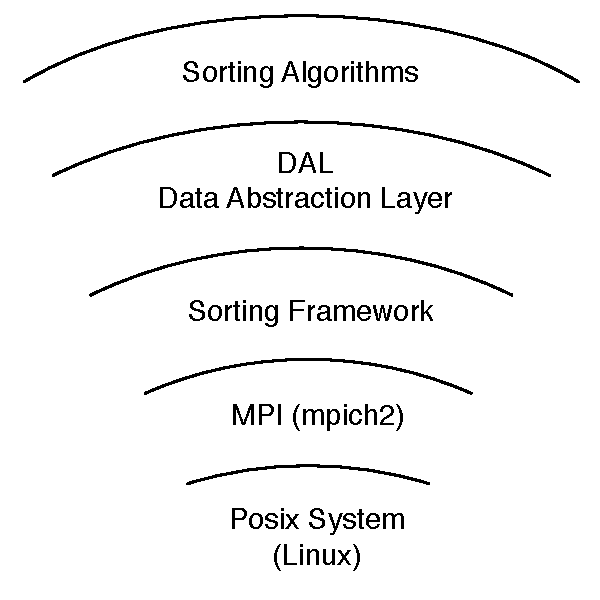
\includegraphics[scale=0.50]{levels}
  \end{center}
  \caption{Our abstract model}
  \label{levels}
\end{wrapfigure}

At this porpose we decided to add a further abstraction layer below the actual sorting algorithm: we decided to introduce a new data structure called \texttt{Data} that represents a dataset indipendently on its form or position: it can represent both an array allocated on principal memory or a file allocated on the hard disk, and it has been thought to be able to represent even other kind of data representation (eg: a compressed dataset). The sorting algorithm, which is our higher abstraction level, doesn't need to know about how or where \texttt{Data} is allocated, and use it in a transparent way.
We needed to write some kind of run-time support for this level, which is logically placed just below the algorithm sorting: since we want to save the algorithm from actually care about how Data is allocated, it needs to use some functions that will take care of it exposing a data-independent signature. Our rule of thumb is that all and only the functions logically placed at this abstraction level are the only ones actually working with a \texttt{Data} object (ie: accessing its field directly or indirectly) and vice-versa.
Functions at this abstraction level will one (or more) \texttt{Data} object, will see wether it's allocated on primary or secondary memory, and according to this they'll run some data-dependent codes, optimized for the medium where the \texttt{Data} object is allocated.


%\subsubsection*{TODO}
%Di che altro c'e' da parlare?
%\begin{itemize}
%	\item{Come funziona piu' nel dettaglio il framework e/o gli algoritmi tenendo conto del data?}
%	\item{Come sono implementati (in via generale/con quale logica -- e/o anche nello specifico) gli algoritmi al livello data?}
%	\item{Il fatto che abbiamo dovuto astrarre MPI?}
%	\item{DOBBIAMO far capire che sta cosa non e' banale, che c'e' costata sangue! non sono riuscito ad essere meno mite di quant'ho scritto...}
%\end{itemize}



\subsection{Sorting Framework}
\subsection*{Data generation}
\subsection*{API}

\section{Performance evaluation}

\subsection{Performance measurement approach}
\label{test-env}
There are two different common approaches to evaluate performance: profiling and benchmarking.

Profiling is used to measure the performance of a given application by adding time measuring and logging code. After the execution has been completed, one can retrace and check how much time had been spent in which function call. This is useful for application developers to find potential bottlenecks and inefficient implemented functions.

Benchmarking addresses mainly the levels underneath the application level, for instance the performance
of the MPI-implementation, the performance of the network and devices. Most interesting results are latencies and bandwidths and their course for various packet or messages sizes. Benchmarking is done by performing numerous iterations of computation and/or communication and measuring the elapsed time.

We used the latter technique to measure the performance of MPI on our test environments, and a combination of both benchmarking and profiling techniques to measure the performance of the different sorting algorithms.

\subsection{Test environment}
In this section we briefly discuss the architecture of our test environments. 

\paragraph{Pianosa}
\textit{Pianosa} is an old cluster of 30 nodes located at the Department of Computer Science, University of Pisa. Nodes are Intel Pentium III 800 Mhz with a L1 cache of 512KB. The primary memory is of size 1 GB. The operative system is an old distribution of Linux, the Fedora Core 1. On average, the available space on disk in each machine is roughly 15 GB; this capacity obviously limits our tests to data sets of relatively small size. The interconnection network between nodes is a Fast Ethernet, so the MPI support is built on top of the stack TCP/IP. The main weakness of the whole architecture is that the interconnection network is based on a hub: the conflicts at network level becomes not negligible, specially for messages of significative size. This is not just an hyphotesis, but something concrete which has been experienced by the group of Parallel Architectures when attempting to define a cost model of MPI. Anyway, even if the architecture has a lot of limitations that can \textit{significantly} affect the performance, Pianosa is a good starting point for testing our algorithms (even from a functional point of view) and to conjecture which architectual characteristics could impair the performance of a Parallel Sorting Algorithm.

\paragraph{PCM}
\label{PCM}
The second target architecture is a cluster of Intel Xeon X5670 (2,93 Ghz) machines located at the Department of Physics, University of Pisa. Each node has 12 cores splitted in 2 chips (6 cores/chip) and each core allows the execution of two simultaneous threads. Each core has both a L1 cache of 64KB (32 KB dedicated to instructions, 32KB to datas) and L2 cache of 256KB. Each chip has also a L3 cache of 12MB, thus shared by 6 cores. The primary memory is of size 48GB. The disk subsystem is 1x1000 GB SATA II, 7200 RPM, surely faster than the one of Pianosa. The operative system is the SUSE Linux Enterprise Server 11. Nodes are interconnected by means of Infiniband; obvioulsy, we will use a version of MPI that supports Infiniband. It is clear that there cannot be comparison between the old Pianosa and this cluster: the newer hardware of this architecture will play a key role for the performance of our Sorting Algorithms, both from a quantitative (absolute time completion) and qualitative (scalability) point of view. We will detail all these aspects in the following sections.

\subsection{Cost Model of MPI}
\label{MPI-cost-model}
\paragraph{The cost of sending a message: the T$\_$send model}
We are interested in evaluating the cost of communications in the test environments because it can help us in understanding the performance behaviour of the Sorting Algorithms. Indeed, depending on both the specific architecture and the algorithm, communications may significatively impact the completion time (and so even the scalability) of the algorithm itself. In a simplified view, the cost of sending a message between two tasks located on different processors can be represented by two parameters: the message startup time $T_{setup}$, which is the time required to initiate the communication, and the transmission time $T_{trasm}$ per word, which is mainly determined by the physical bandwidth of the communication channel linking the source and destination processors~\cite{VANN}. In this model, the time required to send a message of size $L$ (that is, for performing a $DAL\_send$ of size $L$) words is then
\[
T_{send}(L) = T_{setup} + L \times T_{trasm}
\]
While accurate for some algorithms and on very simple architectures, this model generally breaks down due to a lot of factors: for instance, the communication pattern of the application, the bandwith of the interconnection network and, more in general, due to the complexity of the parallel architectures. Despite its weakness, for practical reasons we will refer to the $T\_send$-model to explain the results we achieved.  
The following experimental analysis will try to estimate $T\_send$ on our test architectures by varying the size of the messages and by changing the communication pattern (we will perform the so called ''bisection test'', whichin there are two sets of processes, with same cardinality, that exchange messages each other). 

In order to benchmark the performance of the two environments, we decided to use the \textit{Perftest} benchmark suite.

The perftest-package is provided along with the MPI-implementation MPICH, although it can be used in combination with any MPI-implementation. The package contains a few tools to measure the performance of a message passing environment. The two major programs are \textit{mpptest} for measuring point-to-point communication and \textit{goptest} for measuring collective communication. In addition to the classic ping-pong test, mpptest can measure performance with many participating processes (exposing contention and scalability problems) and can adaptively choose the message sizes in order to isolate sudden changes in performance. 

The following test were performed:
\begin{itemize}
	\item Round-trip times between 2 nodes using blocking methods
	\item Blocking bisection times involving from 4 to $n$ nodes
	\item Broadcast times involving from 2 to $n$ nodes
\end{itemize}
In the bisection test the complete system is logically divided into two subsystems and the aggregated bandwidth and latency between the two subsystems is measured. An example of this is splitting the system in two vertically and letting each node in the left half communicate with a node in the right part on a one-to-one basis.

\paragraph{Optimum size of the DAL's communication buffer}
As we said in section~\ref{DAL-impl} we are interested in estimating the \textit{optimum size} for the communication buffer of the DAL layer. In particular, let's assume that we are performing a $DAL\_send$ of $L$ words. We may have to send these $L$ words either by performing a single $MPI\_Send$ or, more in general, by performing $X$ $MPI\_Send$. The latter situation is not unusual in our framework due to the structure of the DAL layer. Indeed, from section~\ref{DAL-impl}, we remind that each process has its own buffer dedicated to MPI-communications, and this buffer is of fixed size, let's say $K$ words. Since in general $K < L$, assuming without loss of generality that $L = K \times X$, the cost of sending $L$ words is equal to the cost of performing $X$ $MPI\_Send$ each of size $K$. For each architecture, we have to choose the best value of $K$: indeed, a low value may negatively impact on $T\_send$ (because of the setup cost of each $MPI\_Send$); a high value could be useless because a too large communication buffer may not give any benefit, rather it may only constitue a waste of important memory. In order to find the optimal value of $K$, namely the size of the ''static'' communication buffer, we developed a set of utilites (program and script that goes under the name of \textit{Tsetup}) that practically estimates $T\_send$ as function of $L$ and $X$. 

\paragraph{MPI on Pianosa}
\label{test-env-pianosa}
Figures~\ref{pianosa-mpi-1},~\ref{pianosa-mpi-2},~\ref{pianosa-mpi-3} show the cost of $T\_send$ obtained on Pianosa. We will refer to these Figures in the following, when we will explain the performance analisys of the algorithms.

\begin{figure}[p]
	\centering
  	\subfloat[Messages of length from 0 to 32 bytes (stride 4 bytes).]{\label{tsend_32}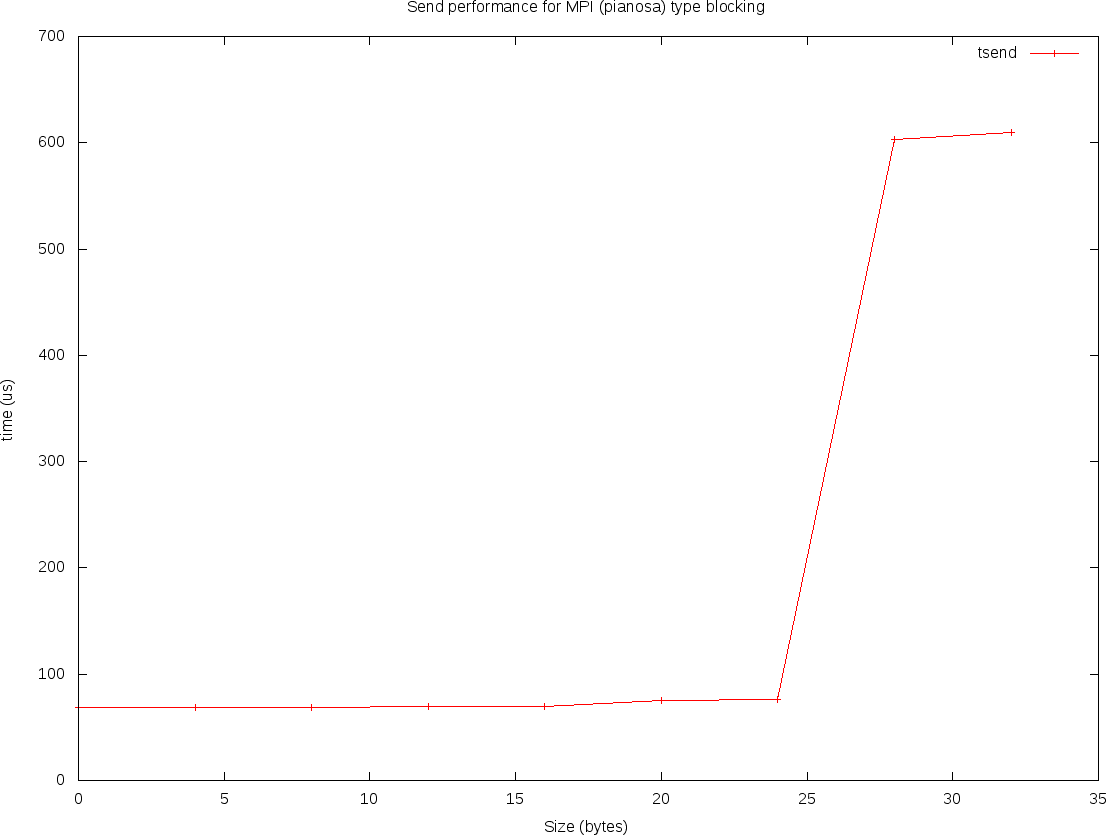
\includegraphics[width=0.4\textwidth]{../tests/mpi_comm_perf/pianosa/tsend_4}}  
	\hspace*{20pt}
  	\subfloat[Messages of length from 0 to 1024 bytes (stride 32 bytes).]{\label{tsend_32}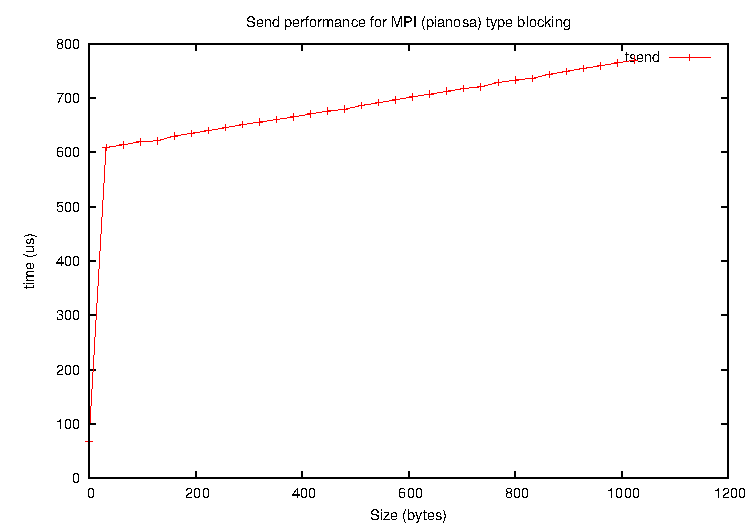
\includegraphics[width=0.4\textwidth]{../tests/mpi_comm_perf/pianosa/tsend_32}}  
	\caption{Performance of blocking send between two processes.}
	\label{pianosa-mpi-1}
	
	\centering
  	\subfloat[Messages of length from 0 to 32768 bytes (stride $2^i$ bytes).]{\label{tsend_logscale}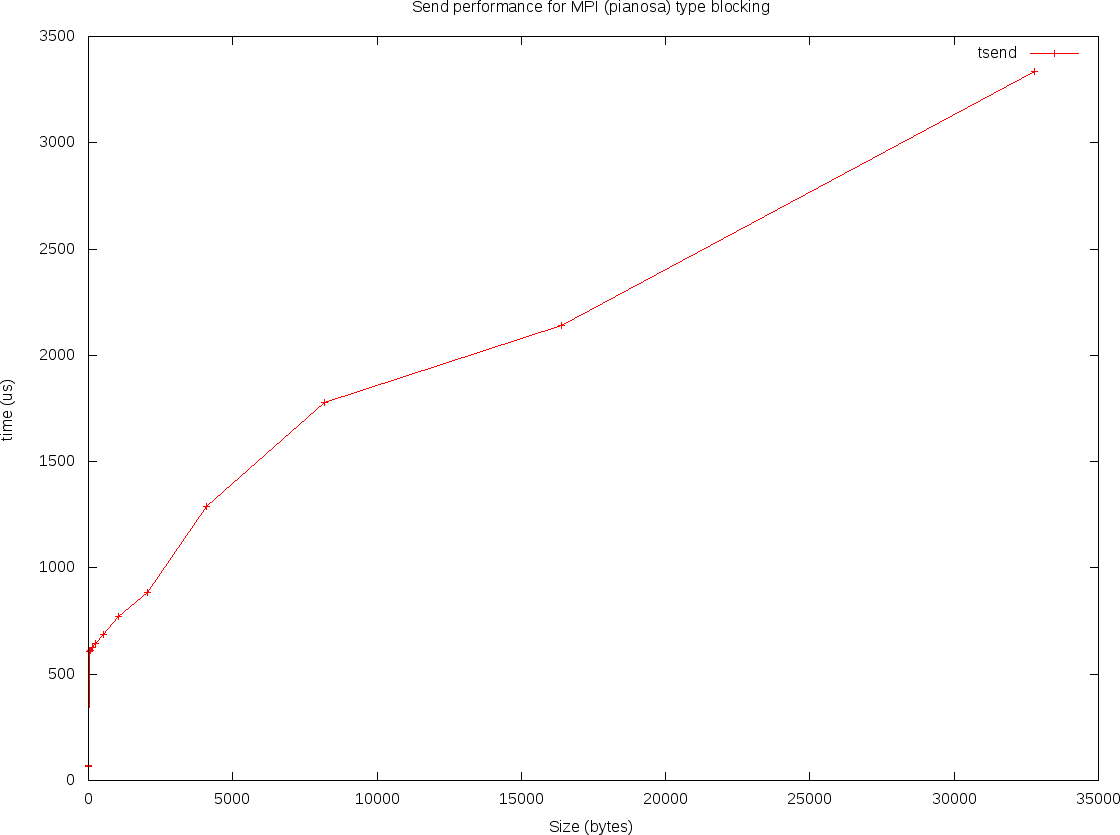
\includegraphics[width=0.4\textwidth]{../tests/mpi_comm_perf/pianosa/tsend_logscale}}  
	\hspace*{20pt}
  	\subfloat[Bisection test with 4, 8 and 16 processors.]{\label{bisect_logscale}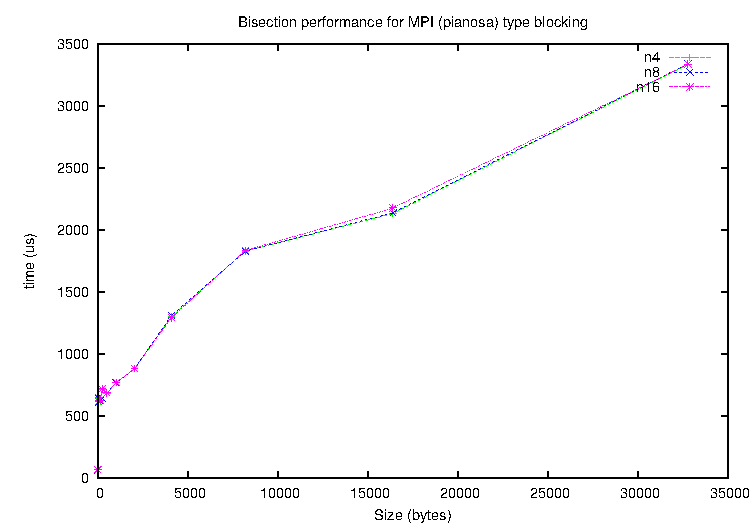
\includegraphics[width=0.4\textwidth]{../tests/mpi_comm_perf/pianosa/bisect_logscale}}  
	\caption{Performance of blocking send and bisection test.}
	\label{pianosa-mpi-2}	
	
	\centering {\label{bcast}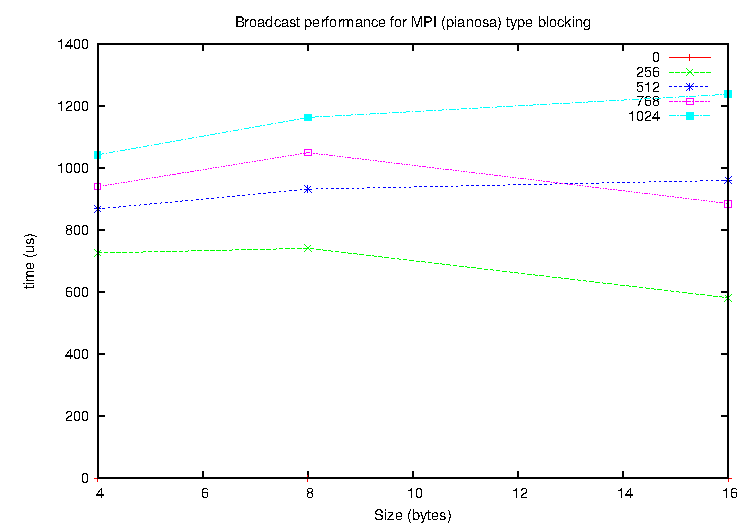
\includegraphics[width=0.4\textwidth]{../tests/mpi_comm_perf/pianosa/bcast}}  
	\caption{Performance of broadcast with 4, 8 and 16 processors.}
	\label{pianosa-mpi-3}
\end{figure}

Now we focus on the size of the communication buffer. Table~\ref{tsetup-impact} shows the cost in seconds of DAL$\_\lbrace send, scatter, alltoall \rbrace$ for a message of size 32MB. The $X$ row of the table show the case in which the original message has been splitted in $X$ $MPI\_\lbrace send, scatter, alltoall \rbrace$, with $X \in \lbrace 2^i : i = 0...18 \rbrace$. TODO: need comment
\begin{table}[h]
\begin{center}
\begin{tabular}{|c|c|c|c|c|}\hline
\hline
$\sharp$ MPI calls & MPI size ($\frac{L}{\sharp Sends}$ bytes)  & $T\_send$   & $T\_scatter$  & $T\_alltoall$      \\\hline\hline
1 & 33554432 & 3.2890 & 3.2557 & 5.4890 \\\hline
2 & 16777216 & 3.2845 & 3.2548 & 5.4769 \\\hline
4 & 8388608 & 3.2847 & 3.2542 & 5.5114 \\\hline
8 & 4194304 & 3.2852 & 3.2549 & 5.4967 \\\hline
16 & 2097152 & 3.2862 & 3.2560 & 5.5235 \\\hline
32 & 1048576 & 3.2867 & 3.2577 & 21.21224 \\\hline
64 & 524288 & 3.2919 & 3.2892 & 26.26160 \\\hline
128 & 262144 & 3.3007 & 3.2829 & 32.31925 \\\hline
256 & 131072 & 3.2847 & 3.2531 & 41.40975 \\\hline
512 & 65536 & 3.2891 & 3.2542 & 72.71889 \\\hline
1024 & 32768 & 3.2854 & 3.2544 & 114.113511 \\\hline
2048 & 16384 & 3.2853 & 3.2553 & 265.265055 \\\hline
4096 & 8192 & 3.2859 & 3.2580 & 15.15112 \\\hline
8192 & 4096 & 3.2868 & 3.2645 & 20.20080 \\\hline
16384 & 2048 & 3.2892 & 3.2790 & 48.47531 \\\hline
32768 & 1024 & 3.2935 & 3.3275 & 84.84000 \\\hline
65536 & 512 & 3.3221 & 4.4270 & 155.154831 \\\hline
131072 & 256 & 4.3956 & 6.6259 & 291.290647 \\\hline
262144 & 128 & 6.5900 & 15.15130 & 573.572866 \\\hline
\end{tabular}
\caption{DAL$\_\lbrace send, scatter, alltoall \rbrace$ cost for messages of size 32MB. }
\label{tsetup-impact}
\end{center}
\end{table}


\paragraph{MPI on Physics}

\subsection{Algorithms Efficiency}
In this section, we are going to analyze the theoretical Algorithm Efficiency defined in~\ref{terminology}. For the sake of commodity, we report here the definition. Given
\begin{itemize}
\item $N$, the parallelism degree; 
\item $m$, the number of steps of the algorithm;
\item $X_i$, a random variable which counts the number of active processes that contribute to the calculation during the step $i$.
\end{itemize}
We defined the Algorithm Efficiency $\varphi$ as:
\begin{center}
$\varphi = \frac{\sum_{i=0}^m E[X_i]}{N \times m} $
\end{center}
In this section we want to give an idea of how many of the $N$ processes with which a Sorting Algorithm is executed are actually exploited by the parallel logic of the algorithm. In the following we show the Algorithm Efficiency of each Sorting Algorithm.

\begin{itemize}
\item \textbf{Mergesort, Quicksort.} $\varphi = \frac{\sum_{i=0}^{ \lceil \log_2{N} \rceil} 2^i}{N \times \lfloor \log_2{N} + 1 \rfloor} $
\begin{enumerate}
\item $N = 16 \rightarrow \frac{31}{80} \approx 0.39$
\item $N = 32 \rightarrow \frac{63}{192} \approx 0.33$
\end{enumerate}

\item \textbf{K-Way Mergesort.} $\varphi = \frac{\sum_{i=0}^{ \lceil \log_k{N} \rceil} min ( k^i, N )}{N \times \lfloor \log_k{N} + 1 \rfloor } $
\begin{enumerate}
\item $N = 16, k = 4 \rightarrow \frac{21}{48} \approx 0.44$
\item $N = 16, k = 8 \rightarrow \frac{25}{48} \approx 0.52$
\end{enumerate}

\item \textbf{Bitonicsort.} $\varphi = \frac{\sum_{i=0}^{(\log_2{N})^2} N}{N \times (\log_2{N})^2} = 1 $
\item \textbf{Bucketsort, Samplesort.} In these algorithms steps have the characteristic of being heterogenous: a first step is the local sorting of datas, than a step of sampling and finally a step for building buckets. A process will never sleep, so we trivialy have: $\varphi = 1$.

\item \textbf{Load Balanced Mergesort, K-Way Load Balanced Mergesort.} Trivialy, $\varphi = 1$. Indeed, these algorithms have been conceived exactly for maximizing the number of processes which contributes to the sorting during all the computation.

\end{itemize}

\subsection{Performance analysis of the algorithms}
\label{performance-analysys}
We said in~\ref{sort-fram} that sorting a data set is a computation described by a \textit{5-tuple} $\langle n$, $M$, $s$, $\Lambda$, $\sigma \rangle$, with $n$ the parallelism degree, $M$ the size of the data set, $s$ a seed for generating the data set, $\Lambda$ the algorithm and $\sigma$ a set of parameters depending on $\Lambda$. In reality, $\sigma$ is significative just for some algorithms; for instance, it can specify the \textit{stencil} (communication pattern) for the processes of a parallel algorithm or the value of ''\textit{K}'' in algorithms like \textit{K-way mergesort}. For each $\Lambda$, we will run single-shot computations (that is, there are not streams of data sets to sort) by varying $n$, $M$, $s$. Initially, $\sigma$ will be fixed for every computations. It is a convention that we will refer to \textit{small}, \textit{large} or \textit{huge} data sets for sizes that are respectively a few MBs, hundreads of MBs and (at least) GBs. 

In order to analyze the performance of the algorithms from different perspective (e.g.: scalability of the specific algorithm, comparison of the time completion required by different algorithms to sort a specific data set and so on) we are going to show different types of graphics. Each graphic is defined by a 3-tuple $\langle x, y, plot \rangle $, where $x$ is the variable on the X axis, $y$ the variable on the Y axis and $plot$ a parameter that identifies a specific shape of that graphic. In particular, given $T$ the time completion of a computation, we will focus on the following graphics:
\begin{enumerate}
\item fixed $M$, a graphic $\langle n, T, \Lambda \rangle $ is necessary to see which is \textit{the ''best'' algorithm} for sorting a data set of a certain $M$ on a specific architecture. Here, we refer to the ''best'' algorithm(s) as the one(s) that is able either to sort faster a specific data set, to scale better or a combination of them. 
\item fixed $\Lambda$, a graphic $\langle n, T, M \rangle$ is useful to see the \textit{scalability} of $\Lambda$ on a specific architecture. Different shapes shows the scalability of $\Lambda$ for different sizes of the data set.
\item fixed $\Lambda$, a graphic $\langle M, T, n \rangle$ to show (as before) the behaviour of $\Lambda$ on a specific architecture, but from a different perspective. 
\item a graphic $\langle M, T, \Lambda \rangle$ to understand which algorithm \textit{should} be used if the target architecture allowed a parallelism degree of at most $n$. These graphics could be used as ''experimental cost models'', in sense that in principle they could predict the performance of a Sorting Algorithm on such architectures that are ''similar'' to our target architectures. Here, ''similar'' refers mainly to CPUs, memory hierarchies, I/O subsystem, interconnection structure.  
\end{enumerate}

The parameters of the computations will take the following values:
\begin{itemize}
\item $\Lambda \in \lbrace$Sequentialsort, Bitonicsort, Samplesort, Bucketsort, Mergesort, Quicksort, K-Way Mergesort, Load-Balanced Mergesort, Load-Balanced Multi-Way Mergesort$\rbrace$;
\item $n \in \lbrace$1, 2, 4, 8, 16, 32, 64, 128, 256$\rbrace$; notice that the maximum value that $n$ can take depends on the specific architecture. 
\item $M \in \lbrace 2^{10 + i} : i = 0, ..., 25\rbrace$ elements (integers). So $M$ takes values from a few kilobytes to tens of gigabytes (recall that each integers is usually represented through 4 bytes).
\end{itemize} 

For each target architecture, first we will focus on analyzing the scalability of each Sorting Algorithms (graphics 2, 3). Then, we will compare them by fixing the size of the data set and showing which algorithm sorts it faster, for different parallelism degrees (graphic 1). Finally, we will show and explain which is the best algorithm for our target architectures. 

\subsubsection{Pianosa}
On this architecture, due to the lack of space on disks, we will be able to test Sorting Algorithms for data sets of size at most 4GB, namely 1G integers. Further, given the results of tests shown in~\ref{test-env-pianosa}, the size of the communication buffer of the DAL layer has been set to 32MB. We have also practically experienced that a larger buffer, in general, does not give significant benefits, while a shorter one impair a little the Time Completion.

\paragraph{Scalability of Sorting Algorithms}
Figures~\ref{NxTxM} and~\ref{MxTxN} show the Time Completion of Sorting Algorithms on Pianosa.

If the data set is \textbf{small} (i.e. of size up to 64MB) there is not any Sorting Algorithms that shows a good scalability. Even worse, if we look at Figure~\ref{NxTxA-small} we notice that by increasing the parallelism degree we obtain an increase of the Time Completion too. In reality, this behaviour is not surprising. The cost of \textit{Sequentialsort} (that is, the cost of the standard \textit{ANSI qsort}, since the data set surely fits the primary memory) for small data sets varies between a few seconds and tens of milliseconds, that is the same order magnitude of $T\_send( \sim KB )$ (see~\ref{test-env-pianosa} for more details). This means that the cost of communications between processes has a significative impact on the final performance of Sorting Algorithms. From a qualitative point of view, the higher the parallelism degree, the higher both the number of communications and the overall time spent in sending datas, so higher is even the overhead introduced by the parallelization. This is why Sorting Algorithms cannot scale and usually exhibit a Time Completion even worse than the one of \textit{Sequentialsort}.

Things are a little bit different when the data set is \textbf{large}, namely when its size is between 128MB and 512MB. Figure~\ref{NxTxM} clearly shows that there is not any algorithm that scales. Bucketsort and Samplesort have a little improvement passing from $n=2$ to $n=4$, but nothing extraordinary. However, if the data set is of 512MB, the parallelization is useful to lower the Time Completion with respect to the one of \textit{Sequentialsort}. Figure~\ref{sequential-pianosa} shows that, for sorting 512 MB, \textit{Sequentialsort} takes roughly 400s, while all Sorting Algorithms, except Quicksort, are able to lower it up to roughly 200s with just $n=4$. Unfortunately, we do not obtain any further improve neither moving from $n=4$ to $n=8$ nor considering a smaller data size (with just $M=256MB$ the parallelizzation gain is not significative). Reasons are quite obvious. From one hand, if we increase the parallelism degree the negative impact of communications is greater than the gain coming from having more computational units (working on smaller partitions).  From the other hand, $M=512MB$ means a jump to an important computational grain: indeed, moving from $n=2$ to $n=4$ guarantees processes to work with a partition of the data set that is still significative; this explains why some Sorting Algorithms shows a gain in terms of Time Completion within this range of processes. If we further increase $n$ up to $16$, processes have to work on smaller partitions, which let the parallelization in some sense useless.

Summarizing, we have just seen that Sorting Algorithms do not scale with data sets of sizes up to a few hundreads of megabytes. Moreover, for small data sets, \textit{Sequentialsort} even outperforms all other parallel algorithms. Reasons of this behaviour are mainly two: the fine grain computation on a few datas \textit{and} the cost of communications, which becomes predominant on a cluster. Now, we focus on \textbf{huge} data sets. Even if the computation is still of fine grain, now each process works with larger partitions of the data set. Besides, notice that in our tests the increment of the data set size is exponential (doubles at each test). This means that processes spend greatly more time in computation than what happened for large data sets. Just as an example, think to two data sets $A$ and $B$, the former of size $\sharp A = 256$ MB, the latter of size $\sharp B = 2$ GB; both of them have to be sort with the same generic Sorting Algorithm. Assume that the parallelism degree is $n=8$. In the first phases of the algorithm, each process works with partitions of sizes respectively $local_A = \frac{\sharp A}{n} = 32$ MB and $local_B = \frac{\sharp B}{n} = 256$ MB. It is clear that a lot of more time is spent just to sort local partitions. If the Sorting Algorithm has a parallel logic such that both the workload keeps balanced among processes and the amount of communications do not overcome the time spent in computations, then a Sorting Algorithm \textit{can} scale. For instance, assume that the Sorting Algorithm in question is the \textit{Samplesort}. During the various steps of the algorithm, processes work with partitions of similar sizes and, except in both the initial scattering and final gathering phases, on average they send $local_{\lbrace A,B \rbrace}$ datas (see~\ref{Samplesort}). On the other hand, assume that the Sorting Algorithm is the \textit{Mergesort}. It is still true that when the data set is $B$, processes have a larger computation phase: but it is also true that the workload tends to be concentrated on a few processes through $log_2{n}$ phases of costly communications (in the best case, a process sends $local_{\lbrace A,B \rbrace}$, while in the final step of the algorithm a process has to send $\frac{\sharp\lbrace A,B\rbrace}{2}$ datas). Therefore, this example shows intuitively how for some Sorting Algorithms (in our case \textit{Samplesort}) the increase of the data set size implies a larger increment of the computation phase with respect to the communication phase, while for other algorithms (in our case \textit{Mergesort}) the workload gets unbalanced after costly phases of communications. This example was necessary to give an idea of why we obtain the behaviour shown in Figure~\ref{NxTxM}, where for huge data sets only some Sorting Algorithms significatively improve their Time Completion by increasing $n$ (\textit{Bucketsort}, \textit{Samplesort}, \textit{Load-Balanced (Multi-Way) Mergesort}, \textit{Bitonicsort}), while other either do not get better (\textit{Mergesort}, \textit{4-Way Mergesort}) or even worsen (\textit{Quicksort}). However, notice that in every case the scalability is far away from the ideality. 

Finally, we observe an interesting behaviour. We consider again the Time Completion of Sorting Algorithms in case of huge data sets. Figure~\ref{NxTxM} shows that algorithms like \textit{Samplesort} (Figure~\ref{NxTxM-samplesort}) and \textit{Load-Balanced Multi-Way Mergesort} (Figure~\ref{NxTxM-lbkmergesort}) exhibit the best gain when the parallelism degree grows from 2 to 4, while by passing to 8 and even worse to 16 the gain tends to diminish. There are no valid reasons to think that with higher parallelism degree the gain restarts to grow. On the other hand, \textit{Bitonicsort} (Figure~\ref{NxTxM-bitonicsort}) does not obtain a significative gain with parallelism degrees up to 8, while passing from 8 to 16 the gain nearly halves. Therefore, it would be interesting to study the behaviour of \textit{Bitonicsort} for higher parallelism degree; this will be our matter of study on another target architecture.

\begin{figure}[t]
	\begin{center}
		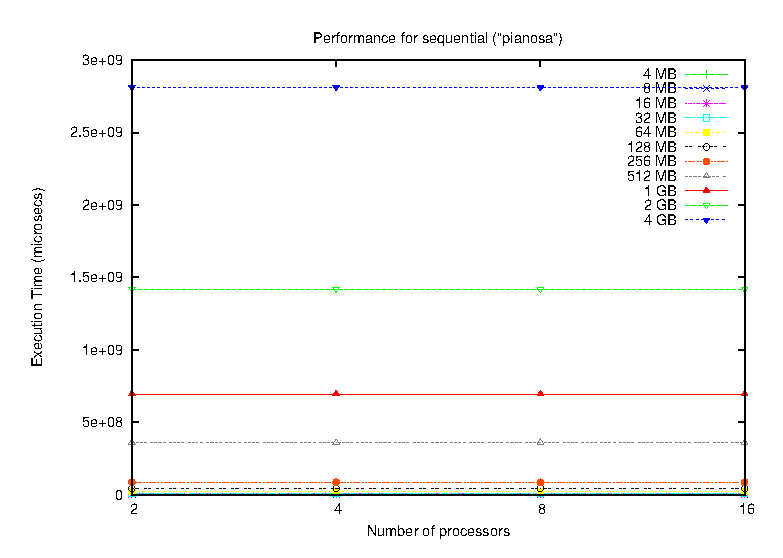
\includegraphics[scale=0.6]{plots/test_01_pianosa/NxTxM/sequential_pianosa_NxTxM}
	\end{center}
  	\caption{\textit{Pianosa}. Completion Time for the Sequentialsort.}
  	\label{sequential-pianosa}
\end{figure}

\begin{figure}[h]
	\centering
	\subfloat[Quicksort.]{\label{NxTxM-sequential}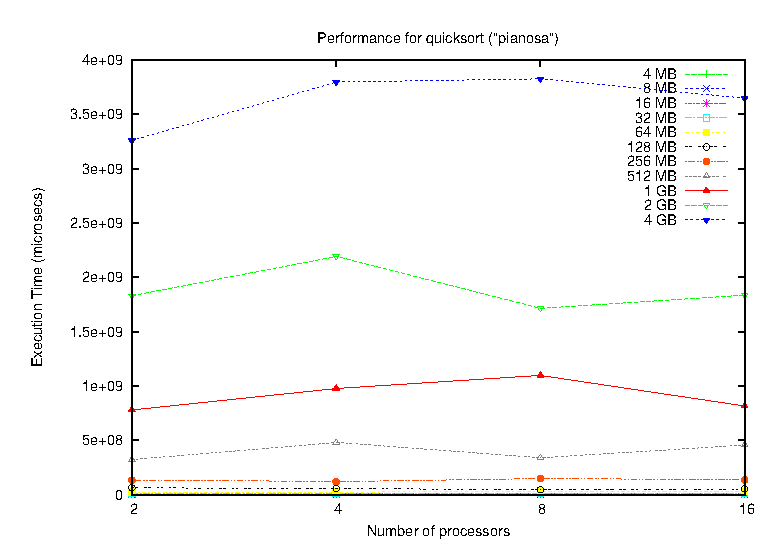
\includegraphics[width=0.4\textwidth]{plots/test_01_pianosa/NxTxM/quicksort_pianosa_NxTxM}} 
	\hspace*{20pt}	
  	\subfloat[Bitonicsort.]{\label{NxTxM-bitonicsort}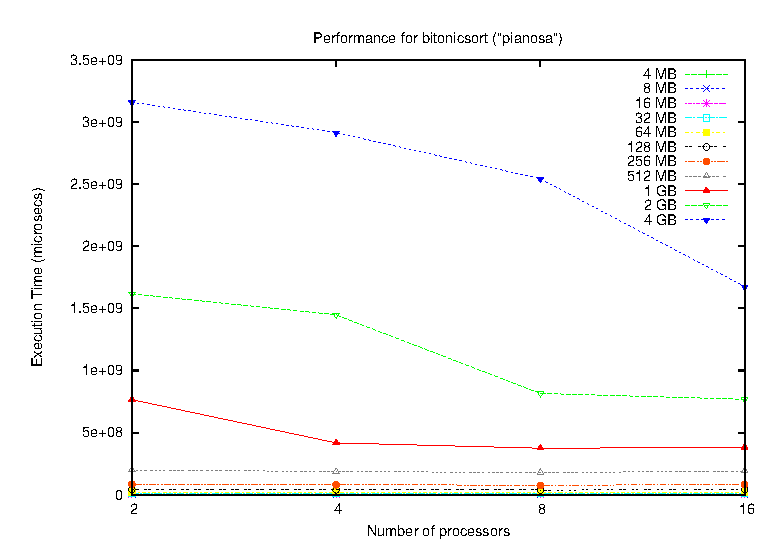
\includegraphics[width=0.4\textwidth]{plots/test_01_pianosa/NxTxM/bitonicsort_pianosa_NxTxM}} 
	
	\centering
	\subfloat[Bucketsort.]{\label{NxTxM-bucketsort}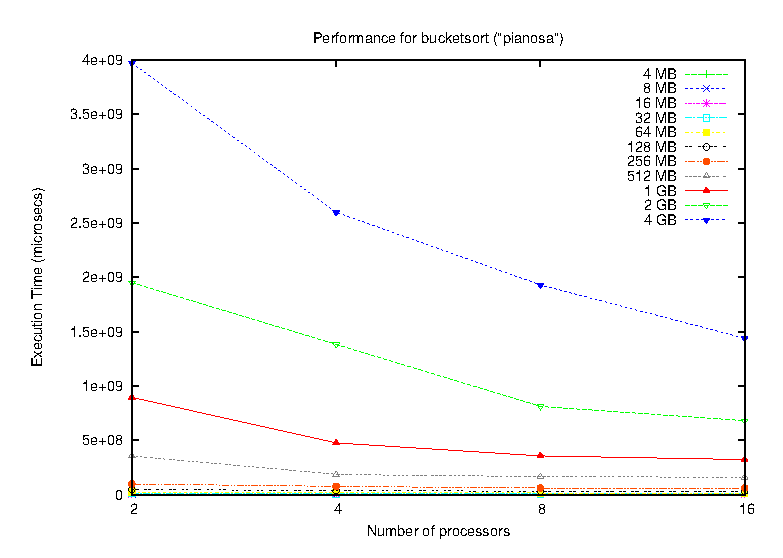
\includegraphics[width=0.4\textwidth]{plots/test_01_pianosa/NxTxM/bucketsort_pianosa_NxTxM}} 
  	\hspace*{20pt}
  	\subfloat[Samplesort.]{\label{NxTxM-samplesort}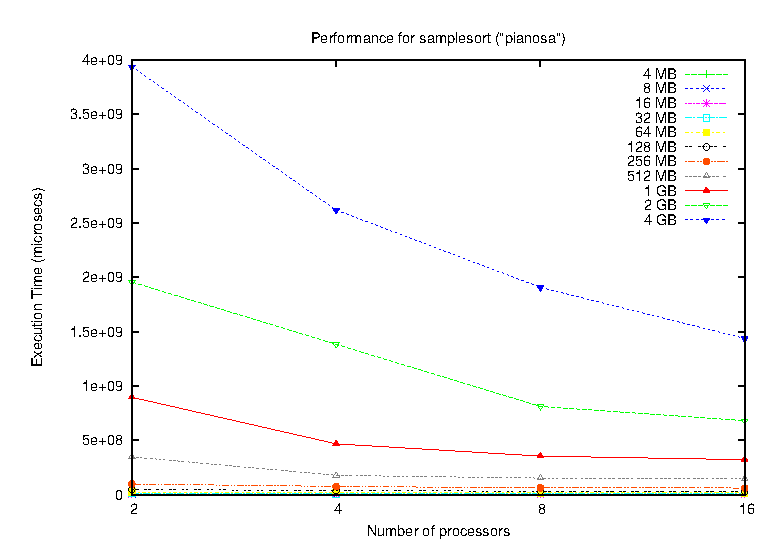
\includegraphics[width=0.4\textwidth]{plots/test_01_pianosa/NxTxM/samplesort_pianosa_NxTxM}} 
	
	\centering
  	\subfloat[Mergesort.]{\label{NxTxM-mergesort}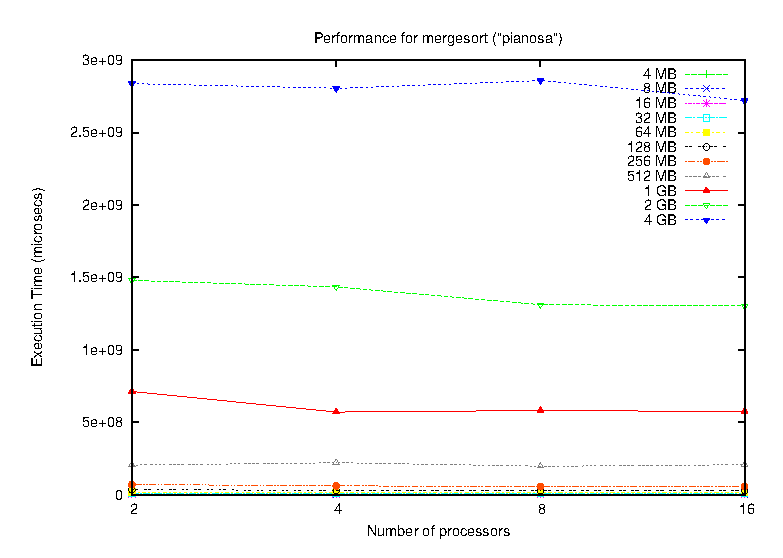
\includegraphics[width=0.4\textwidth]{plots/test_01_pianosa/NxTxM/mergesort_pianosa_NxTxM}}   
  	\hspace*{20pt}  
  	\subfloat[4-Way Mergesort.]{\label{NxTxM-kmerge}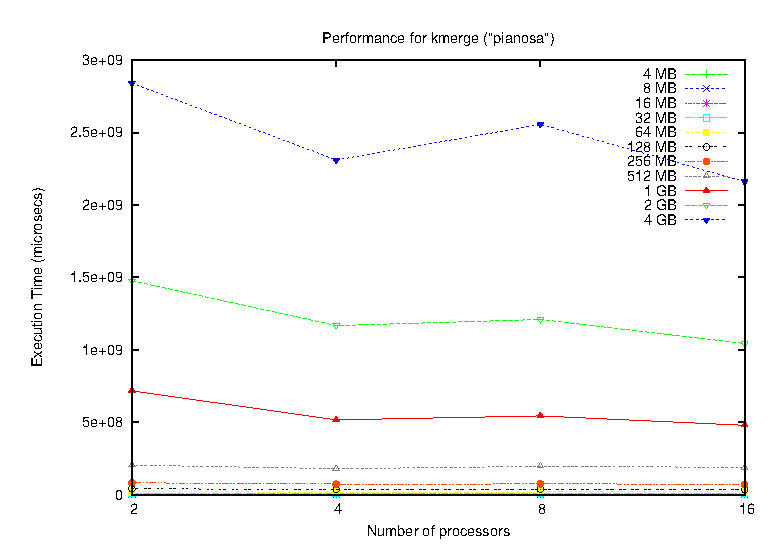
\includegraphics[width=0.4\textwidth]{plots/test_01_pianosa/NxTxM/kmerge_pianosa_NxTxM}} 
	
	\centering
  	\subfloat[Load-Balanced Mergesort.]{\label{NxTxM-lbmergesort}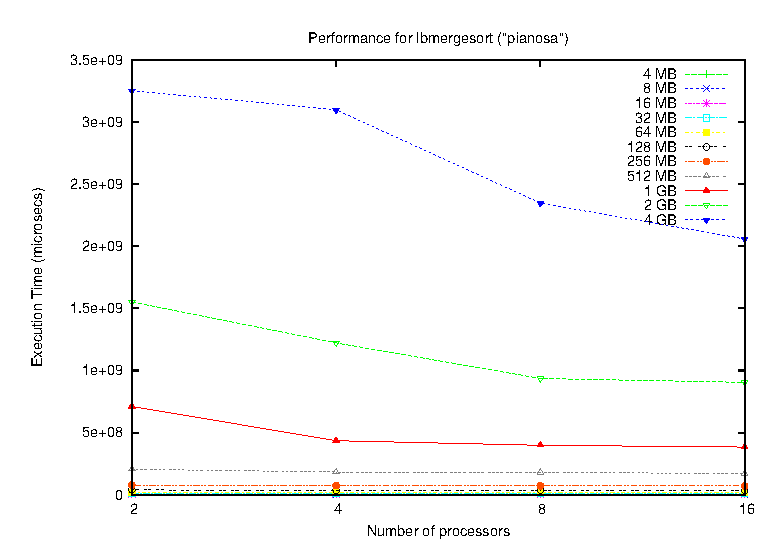
\includegraphics[width=0.4\textwidth]{plots/test_01_pianosa/NxTxM/lbmergesort_pianosa_NxTxM}} 
  	\hspace*{20pt}  
  	\subfloat[Load-Balanced Multi-Way Mergesort.]{\label{NxTxM-lbkmergesort}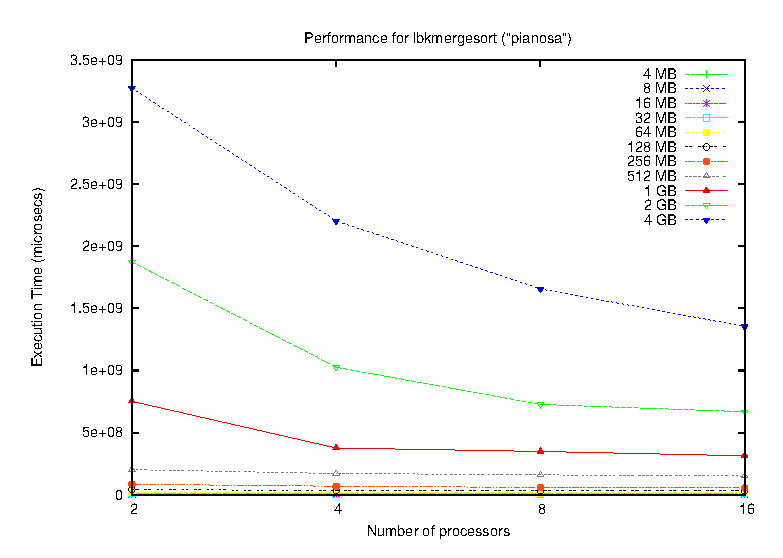
\includegraphics[width=0.4\textwidth]{plots/test_01_pianosa/NxTxM/lbkmergesort_pianosa_NxTxM}} 	
  	
	\caption{\textit{Pianosa}. Time Completion of Sorting Algorithms by varying the parallelism degree. Each shape on a graphic represents the Time Completion of a certain Sorting Algorithm for a data set of specific size.}
	\label{NxTxM}
\end{figure}
 
\begin{figure}[!ht]
	\centering
	\subfloat[Quicksort.]{\label{MxTxN-sequential}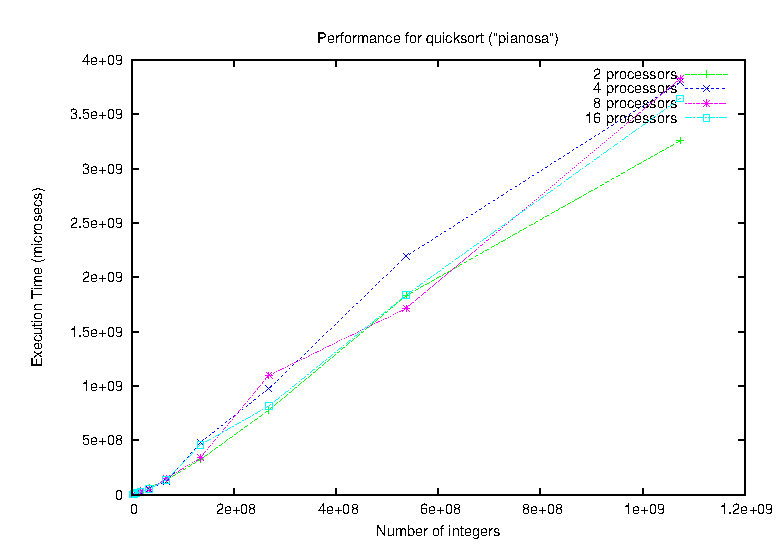
\includegraphics[width=0.4\textwidth]{plots/test_01_pianosa/MxTxN/quicksort_pianosa_MxTxN}} 
	\hspace*{20pt}	
  	\subfloat[Bitonicsort.]{\label{MxTxN-bitonicsort}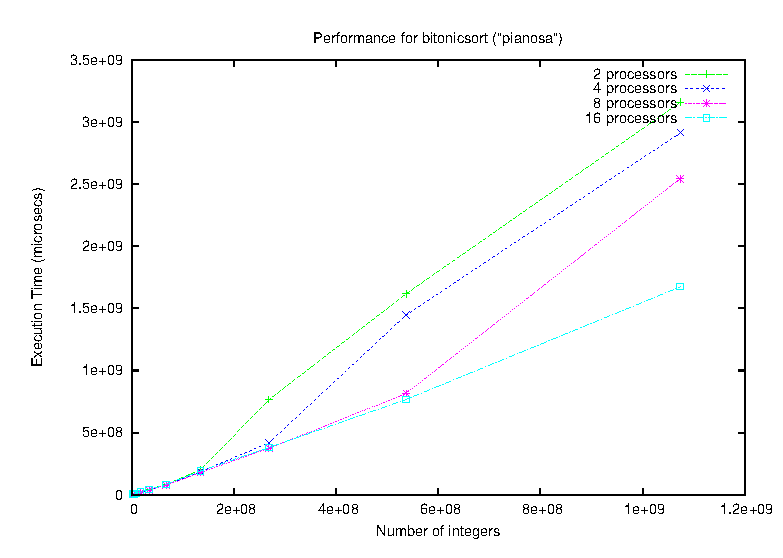
\includegraphics[width=0.4\textwidth]{plots/test_01_pianosa/MxTxN/bitonicsort_pianosa_MxTxN}} 
  		
	\centering
	\subfloat[Bucketsort.]{\label{MxTxN-bucketsort}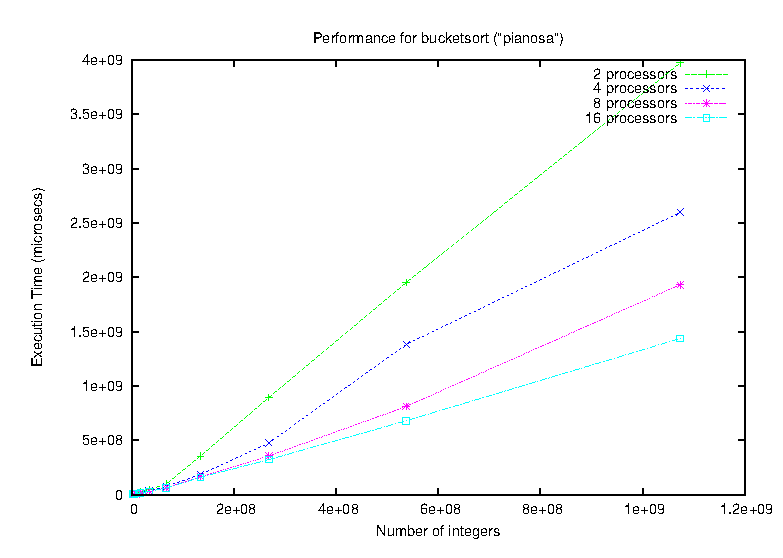
\includegraphics[width=0.4\textwidth]{plots/test_01_pianosa/MxTxN/bucketsort_pianosa_MxTxN}} 
  	\hspace*{20pt}
  	\subfloat[Samplesort.]{\label{MxTxN-samplesort}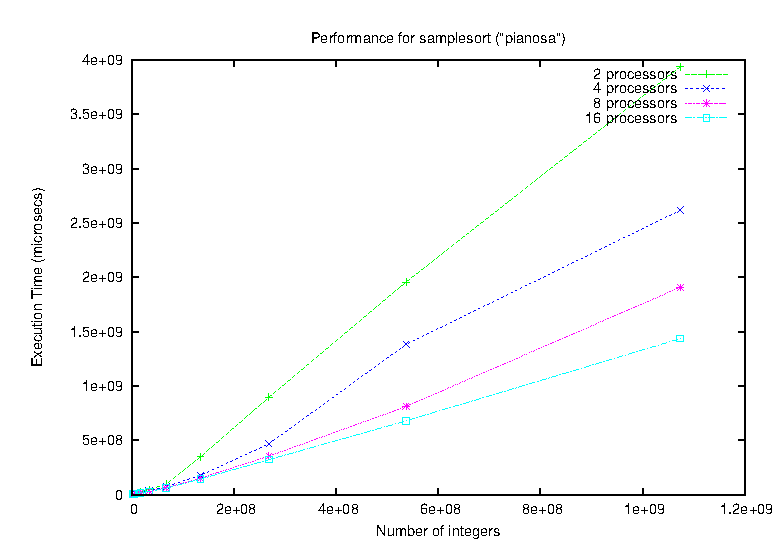
\includegraphics[width=0.4\textwidth]{plots/test_01_pianosa/MxTxN/samplesort_pianosa_MxTxN}} 
	
	\centering
  	\subfloat[Mergesort.]{\label{MxTxN-mergesort}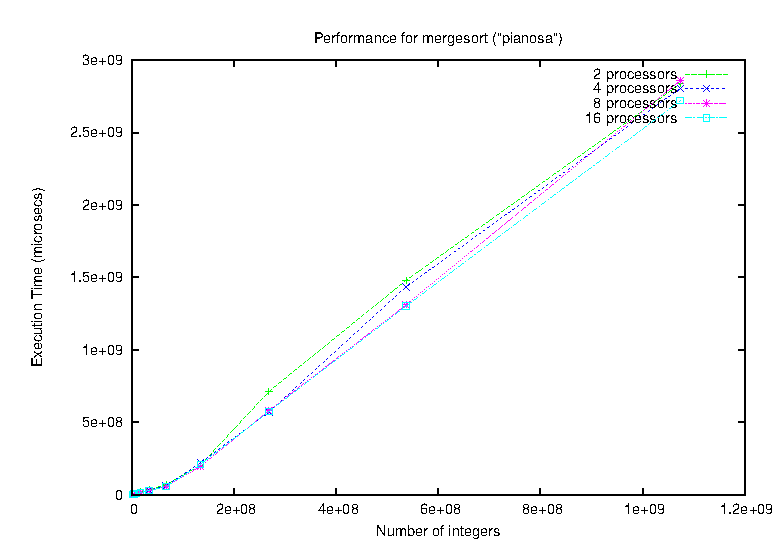
\includegraphics[width=0.4\textwidth]{plots/test_01_pianosa/MxTxN/mergesort_pianosa_MxTxN}}   
  	\hspace*{20pt}  
  	\subfloat[4-Way Mergesort.]{\label{MxTxN-kmerge}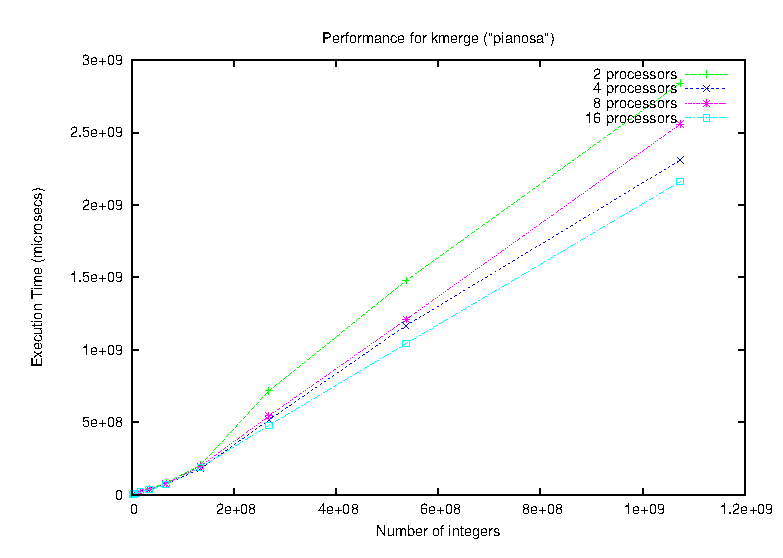
\includegraphics[width=0.4\textwidth]{plots/test_01_pianosa/MxTxN/kmerge_pianosa_MxTxN}} 
	
	\centering
  	\subfloat[Load-Balanced Mergesort.]{\label{MxTxN-lbmergesort}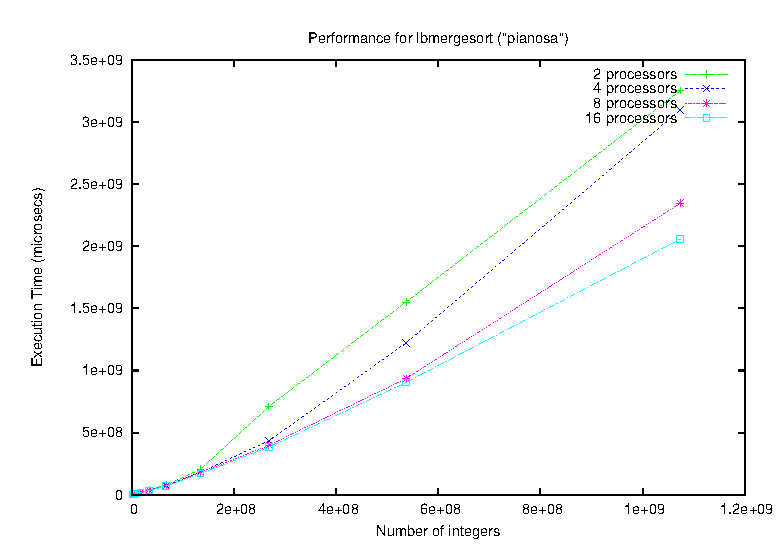
\includegraphics[width=0.4\textwidth]{plots/test_01_pianosa/MxTxN/lbmergesort_pianosa_MxTxN}} 
  	\hspace*{20pt}  
  	\subfloat[Load-Balanced Multi-Way Mergesort.]{\label{MxTxN-lbkmergesort}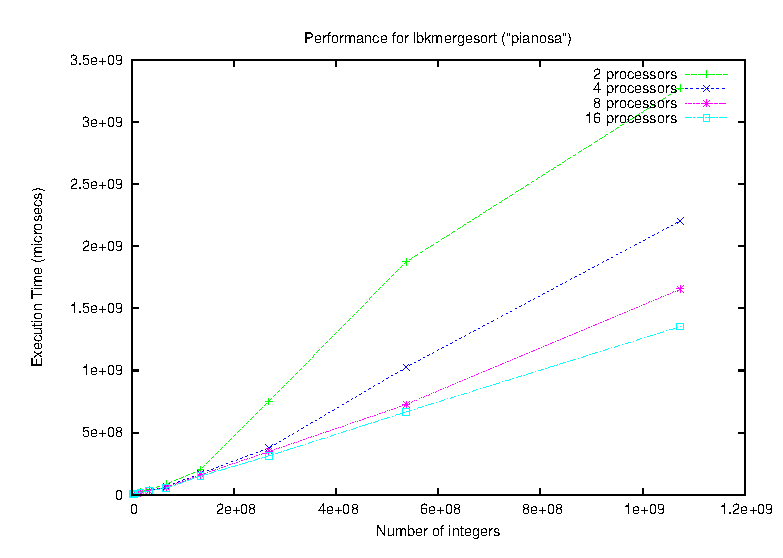
\includegraphics[width=0.4\textwidth]{plots/test_01_pianosa/MxTxN/lbkmergesort_pianosa_MxTxN}} 
  	
	\caption{\textit{Pianosa}. Time Completion of Sorting Algorithms for increasing sizes of the data set. }
	\label{MxTxN}
\end{figure} 
  
\paragraph{Comparison between Sorting Algorithms}
In the previous section we have analyzed the scalability of singles Sorting Algorithms for different sizes of the data set. Now, we focus on determining the best Sorting Algorithm, in terms of Time Completion, for different sizes of the data set. First of all, recall that whether a data set fits the primary memory, a call to \textit{Sequentialsort} is simply a call to the standard \textit{ANSI qsort} (see chapter~\ref{sort-fram}). Therefore, in case of \textbf{small} data sets, the \textit{Sequentialsort} is the best algorithm we can use. Indeed, as we have already anticipated, in these cases the overhead of the parallelization is greater than the time that we would spend in a sequential, optimized computation, like the one of \textit{qsort}. On the other hand, things are obvioulsy different for larger data sets. Figures~\ref{NxTxA-large} and~\ref{NxTxA-huge} can be used to derive which algorithms exhibit the best Time Completions respectively for large and huge data sets. First, we consider the case of \textbf{large} data sets. 
Aside the \textit{Quicksort}, which suffers the unbalancing of the load among processes (see Appendix~\ref{appendix} for more details), most of the Sorting Algorithms outperform \textit{Sequentialsort}, at least when the size of the data set is greater than 4M integers. At least up to parallelism degree 16, the best algorithm is \textit{Mergesort}: in the best case, it is able to lower the Time Completion of \textit{qsort} of roughly 25$\%$ (see Figure~\ref{NxTxA-32M}). Now, we move to \textit{huge} data sets. It has been a great pleasure to see that the \textit{Load-Balanced Multi-Way Mergesort} (the Sorting Algorithm we designed and implemented by taking cue from \textit{Load-Balanced Mergesort}) is the algorithm that shows \textit{always} the best Time Completion (see also Figures~\ref{MxTxA-n4},~\ref{MxTxA-n8} and~\ref{MxTxA-n16}). Unfortunately, the lack of further machines to increase the parallelism degree at least up to 32 prevents the possibility of claiming deeper conclusions on these aspects. 


\begin{figure}[!ht]
	\centering
	\subfloat[Data set of 1M integers.]{\label{NxTxA-1M}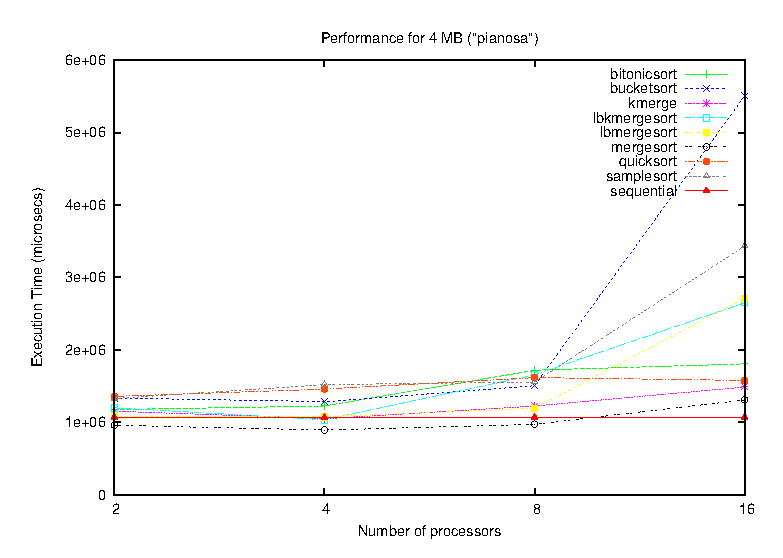
\includegraphics[width=0.4\textwidth]{plots/test_01_pianosa/NxTxA/M1048576_pianosa_NxTxA}} 
	\hspace*{20pt}	
  	\subfloat[Data set of 2M integers.]{\label{NxTxA-2M}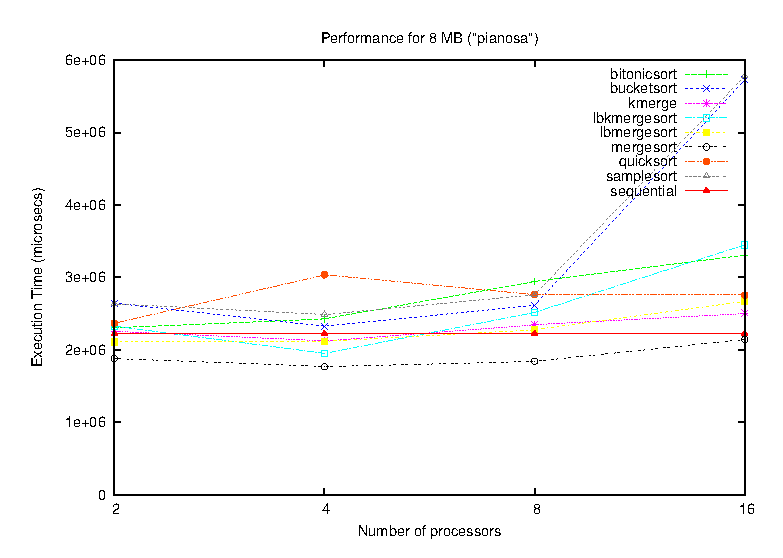
\includegraphics[width=0.4\textwidth]{plots/test_01_pianosa/NxTxA/M2097152_pianosa_NxTxA}} 
  		
	\centering
	\subfloat[Data set of 4M integers.]{\label{NxTxA-4M}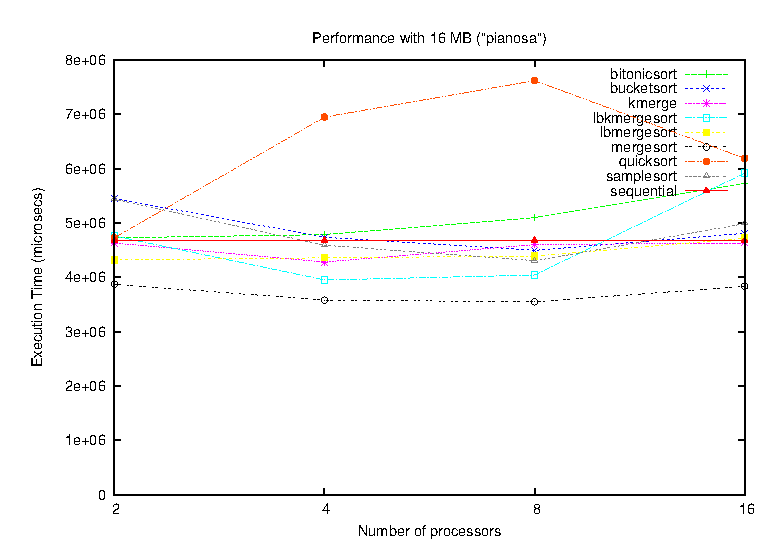
\includegraphics[width=0.4\textwidth]{plots/test_01_pianosa/NxTxA/M4194304_pianosa_NxTxA}} 
  	\hspace*{20pt}
  	\subfloat[Data set of 8M integers.]{\label{NxTxA-8M}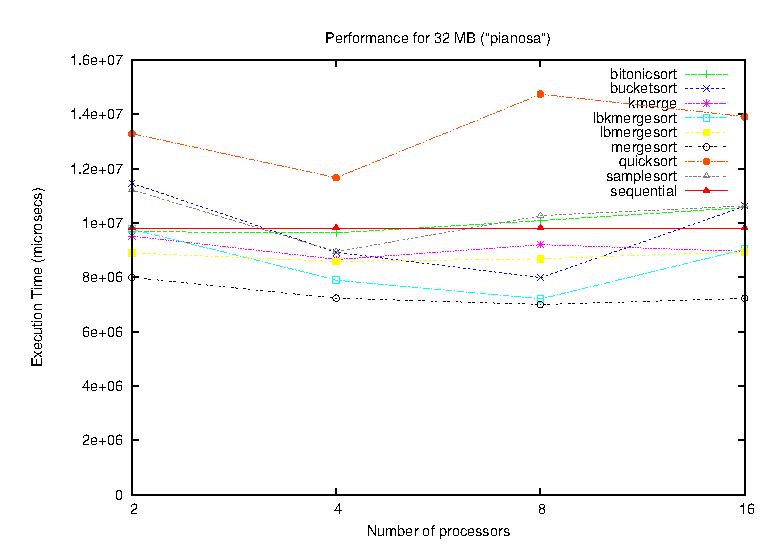
\includegraphics[width=0.4\textwidth]{plots/test_01_pianosa/NxTxA/M8388608_pianosa_NxTxA}} 
	
	\centering
  	\subfloat[Data set of 16M integers.]{\label{NxTxA-16M}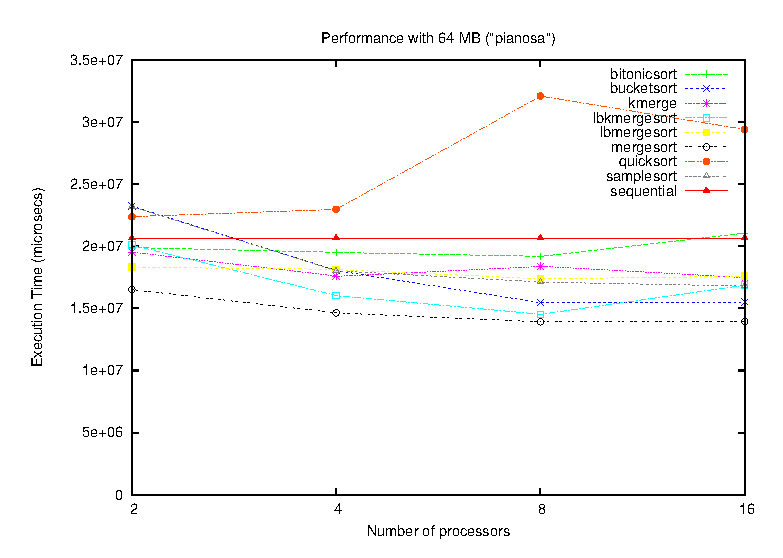
\includegraphics[width=0.4\textwidth]{plots/test_01_pianosa/NxTxA/M16777216_pianosa_NxTxA}}   
  	\hspace*{20pt}  
  	\subfloat[Data set of 32M integers.]{\label{NxTxA-32M}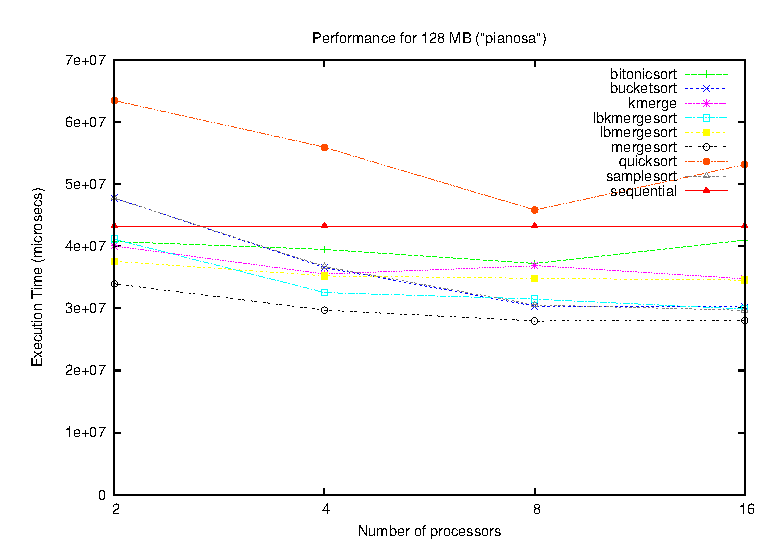
\includegraphics[width=0.4\textwidth]{plots/test_01_pianosa/NxTxA/M33554432_pianosa_NxTxA}} 
  	
	\caption{\textit{Pianosa}. Time Completion for sorting \textit{small} data sets. Each graphic represents a data set of fixed size, while each shape on a graphic shows the Time Completion of a certain Sorting Algorithm for that data set.}
	\label{NxTxA-small}
\end{figure} 

\begin{figure}[!ht]
	\centering
	\subfloat[Data set of 64M integers.]{\label{NxTxA-64M}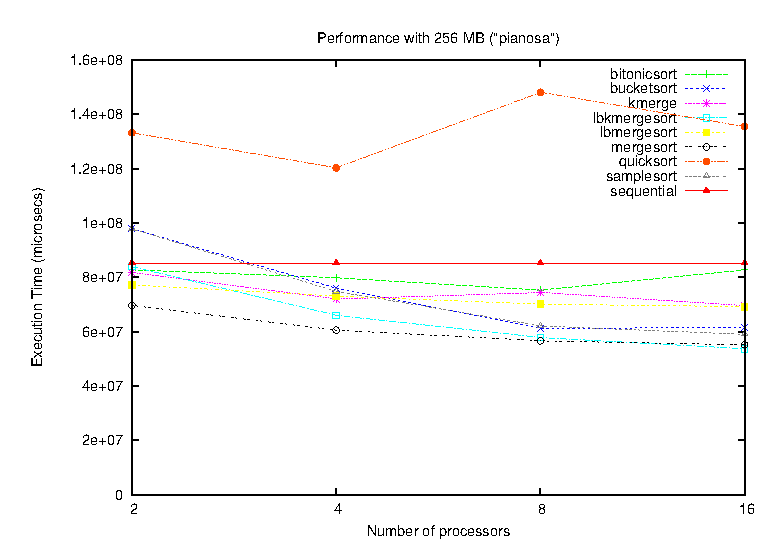
\includegraphics[width=0.5\textwidth]{plots/test_01_pianosa/NxTxA/M67108864_pianosa_NxTxA}} 
	
	\centering
  	\subfloat[Data set of 128M integers.]{\label{NxTxA-128M}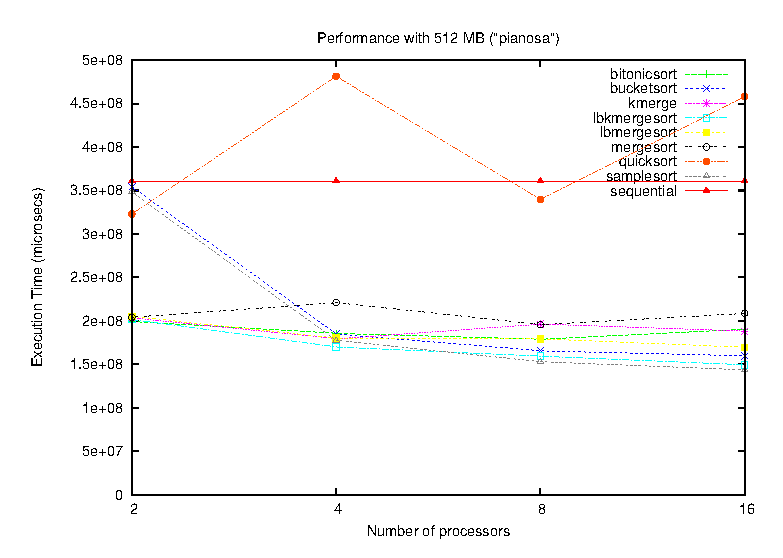
\includegraphics[width=0.5\textwidth]{plots/test_01_pianosa/NxTxA/M134217728_pianosa_NxTxA}} 
  		
	\centering
	\subfloat[Data set of 256M integers.]{\label{NxTxA-256M}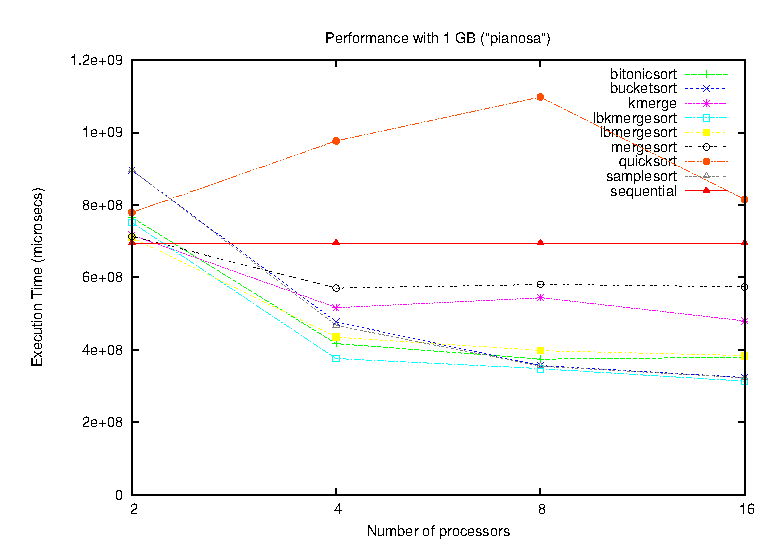
\includegraphics[width=0.5\textwidth]{plots/test_01_pianosa/NxTxA/M268435456_pianosa_NxTxA}} 
  	
  	\caption{\textit{Pianosa}. Time Completion for sorting \textit{large} data sets. Each graphic represents a data set of fixed size, while each shape on a graphic shows the Time Completion of a certain Sorting Algorithm for that data set.}
	\label{NxTxA-large}
\end{figure}

\begin{figure}[!ht]  	
  	\centering
  	\subfloat[Data set of 512M integers.]{\label{NxTxA-512M}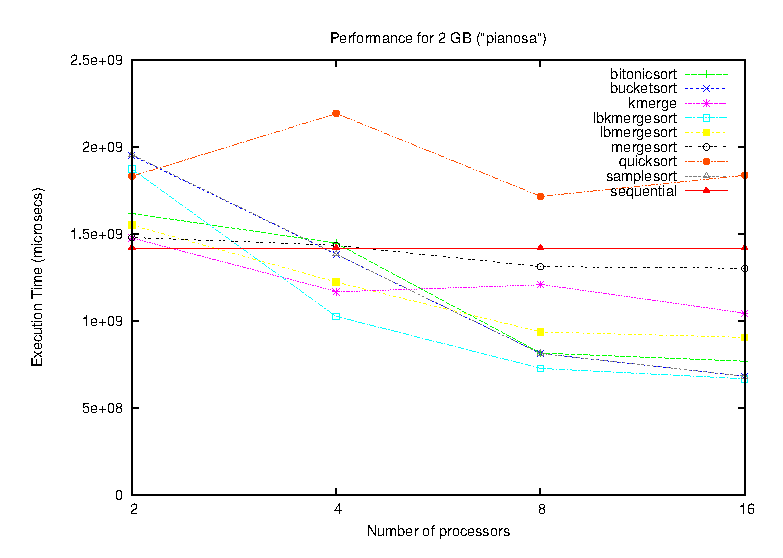
\includegraphics[width=0.6\textwidth]{plots/test_01_pianosa/NxTxA/M536870912_pianosa_NxTxA}} 
	
	\centering
  	\subfloat[Data set of 1G integers.]{\label{NxTxA-1G}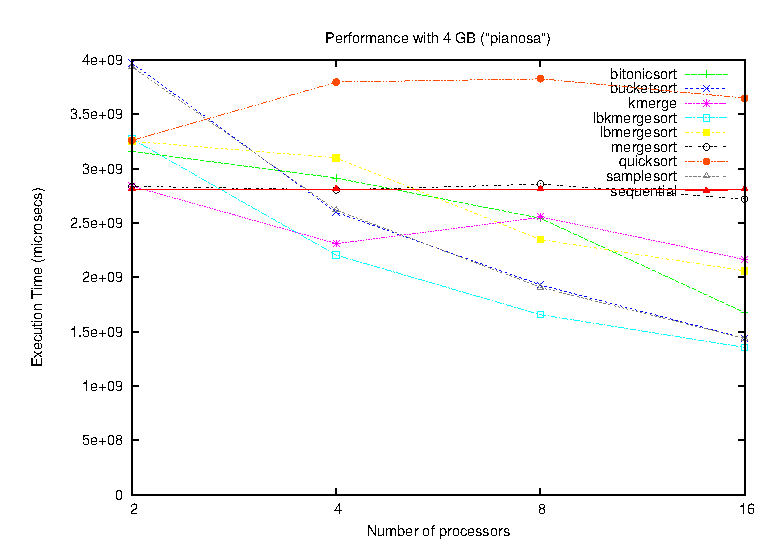
\includegraphics[width=0.6\textwidth]{plots/test_01_pianosa/NxTxA/M1073741824_pianosa_NxTxA}}    
  	
	\caption{\textit{Pianosa}. Time Completion for sorting \textit{huge} data sets. Each graphic represents a data set of fixed size, while each shape on a graphic shows the Time Completion of a certain Sorting Algorithm for that data set.}
	\label{NxTxA-huge}
\end{figure} 

\begin{figure}[!ht]
	\centering
	\subfloat[Parallelism degree 2.]{\label{MxTxA-n2}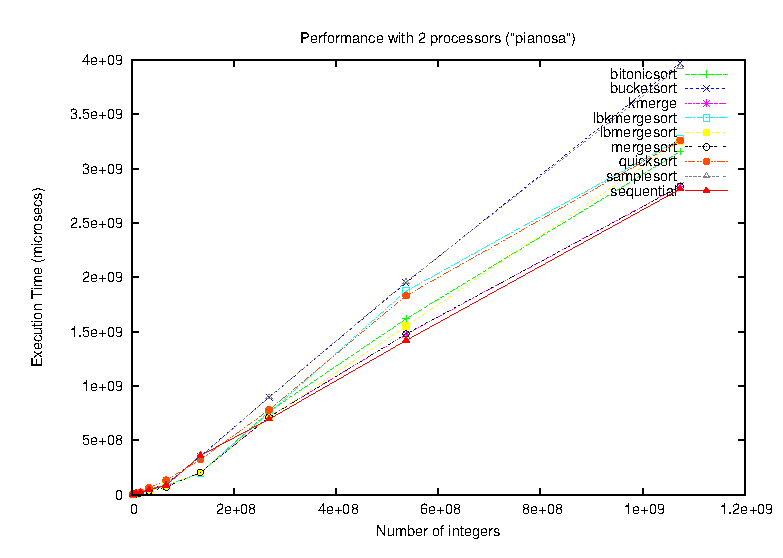
\includegraphics[width=0.4\textwidth]{plots/test_01_pianosa/MxTxA/n2_pianosa_MxTxA}} 
	\hspace*{20pt}	
  	\subfloat[Parallelism degree 4.]{\label{MxTxA-n4}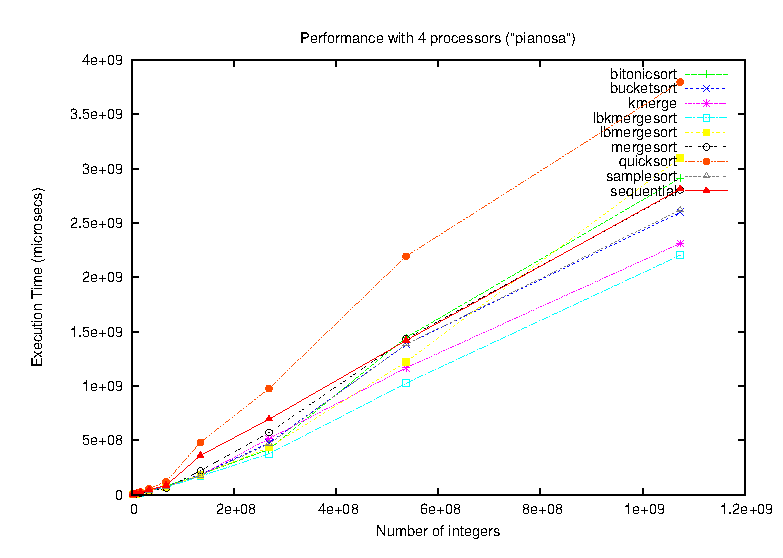
\includegraphics[width=0.4\textwidth]{plots/test_01_pianosa/MxTxA/n4_pianosa_MxTxA}} 
  		
	\centering
	\subfloat[Parallelism degree 8.]{\label{MxTxA-n8}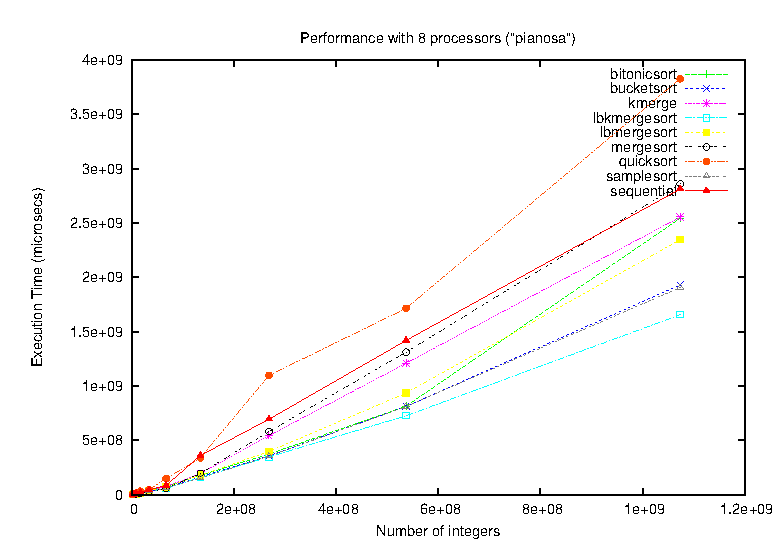
\includegraphics[width=0.4\textwidth]{plots/test_01_pianosa/MxTxA/n8_pianosa_MxTxA}} 
  	\hspace*{20pt}
  	\subfloat[Parallelism degree 16.]{\label{MxTxA-n16}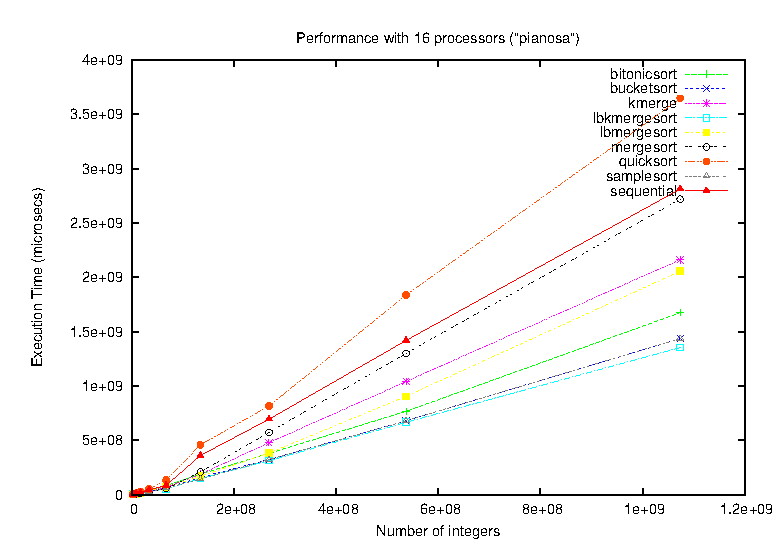
\includegraphics[width=0.4\textwidth]{plots/test_01_pianosa/MxTxA/n16_pianosa_MxTxA}} 
  	
	\caption{\textit{Pianosa}. Time Completion for sorting data sets with fixed parallelism degree.}
	\label{MxTxA}
\end{figure} 

\clearpage
\subsubsection{Intel Xeon X5670}
In this section we analyze the behaviour of Sorting Algorithms on a Chip MultiProcessor (CMP), namely a Symmetric MultiProcessor (SMP) on chip. The CMP in question is the Intel Xeon X5670, described in~\ref{PCM}, which is a generic node of the cluster $PCM$. We will be able to test our algorithms for parallelism degrees up to 8. We expect that performance results on this architecture will be significantly different from the ones obtained on Pianosa, in particular from a \textit{qualitative} point of view. Indeed, there are two key factors: first, the huge amount of primary memory will diminish the overhead due to I/Os; second, the communications now take place in shared memory thus they are less expensive.

\paragraph{Scalability of Sorting Algorithms} Figure~\ref{PCM-NxTxM} and~\ref{PCM-MxTxN} show the time completion of Sorting Algorithms for data sets up to 2 GB. Exactly as on $Pianosa$, due to the fine grain computation, there is not any Sorting Algorithm that shows a good scalability for \textbf{small} data sets. On the other hand, the previous considerations on the primary memory size and the cost of communications justify intuitively why, for \textbf{large} data sets, most Sorting Algorithms scale better than on $Pianosa$ (even if still far away from the ideality). Figure~\ref{PCM-NxTxM} shows that increasing the parallelism degree from 2 to 4, a lot of Sorting Algorithms scale really close to the ideality, while from 4 to 8 there is still a gain, but in general lower. Exactly as on $Pianosa$, \textit{Bucketsort}, \textit{Samplesort} and \textit{Load-Balanced Multi-Way Mergesort} exhibit the best performance in terms of both scalability and time completion. \textit{Mergesort} (Figure~\ref{PCM-NxTxM-mergesort}) was bad on $Pianosa$ because of both the communications overhead and the unbalanced workload, but now exhibit a great scalability up to parallelism degree 8; this is thanks also to the faster hardware which let the last sequential phase of merging becoming less incisive on the overall time completion. Figure~\ref{PCM-NxTxM-quicksort} shows \textit{Quicksort} which has the worst performance TODO. Figure~\ref{PCM-NxTxM-kmerge} shows the bad performance of \textit{4-Way Mergesort}; this algorithm suffers the last phase of merging that, since it is made by a single process (see~\ref{kmerge}), becomes predominant with respect to the gain of the parallelization. 

\begin{figure}[t]
	\begin{center}
		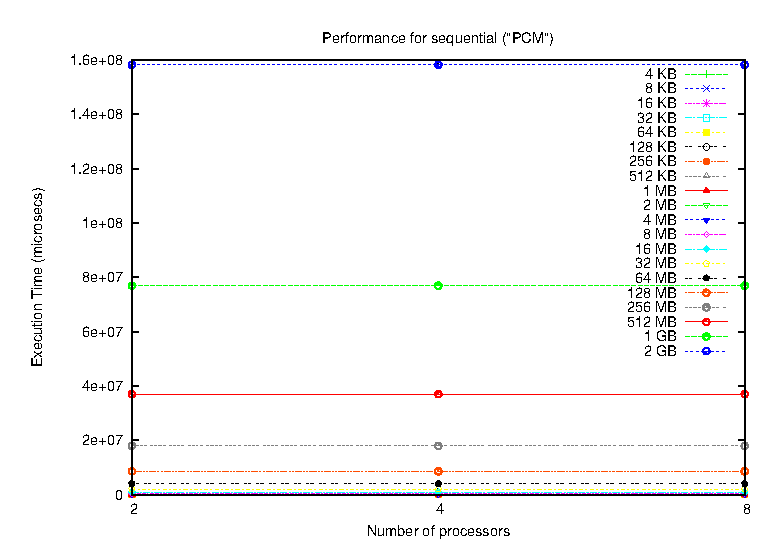
\includegraphics[scale=0.6]{plots/test_00_PCM/NxTxM/sequential_PCM_NxTxM}
	\end{center}
  	\caption{\textit{Intel Xeon X5670}. Completion Time for the Sequentialsort.}
  	\label{sequential-PCM}
\end{figure}

\begin{figure}[h]
	\centering
	\subfloat[Quicksort.]{\label{PCM-NxTxM-sequential}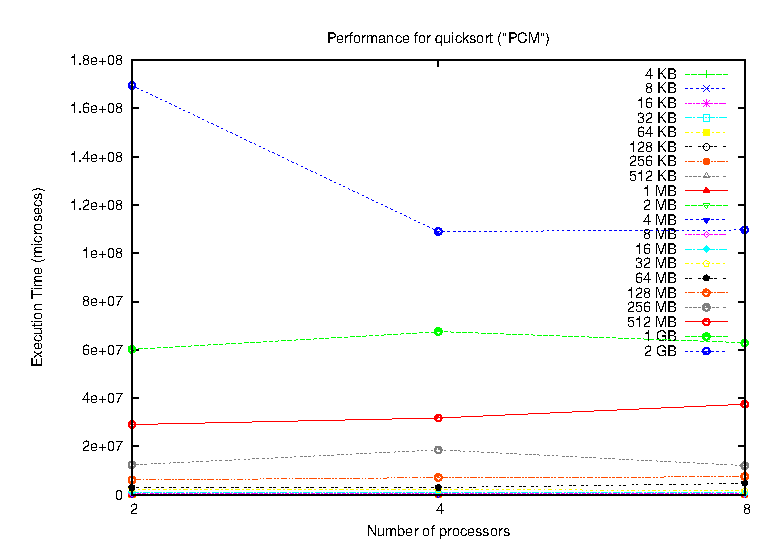
\includegraphics[width=0.4\textwidth]{plots/test_00_PCM/NxTxM/quicksort_PCM_NxTxM}} 
	\hspace*{20pt}	
  	\subfloat[Bitonicsort.]{\label{PCM-NxTxM-bitonicsort}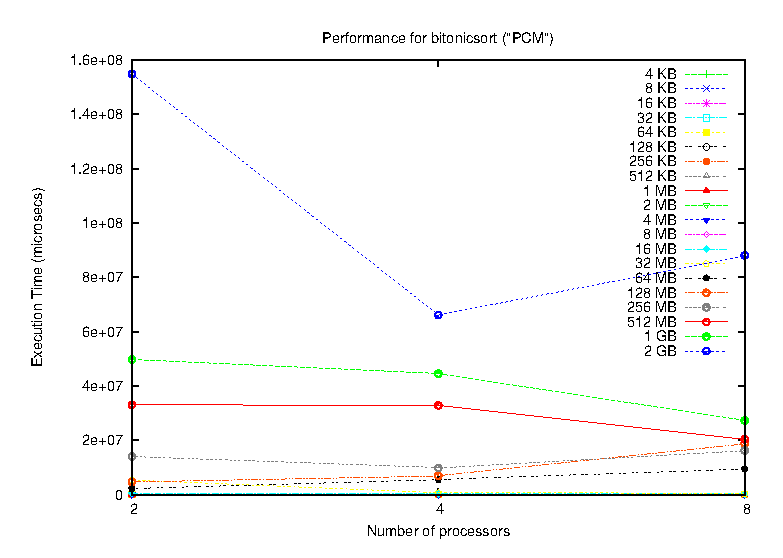
\includegraphics[width=0.4\textwidth]{plots/test_00_PCM/NxTxM/bitonicsort_PCM_NxTxM}} 
	
	\centering
	\subfloat[Bucketsort.]{\label{PCM-NxTxM-bucketsort}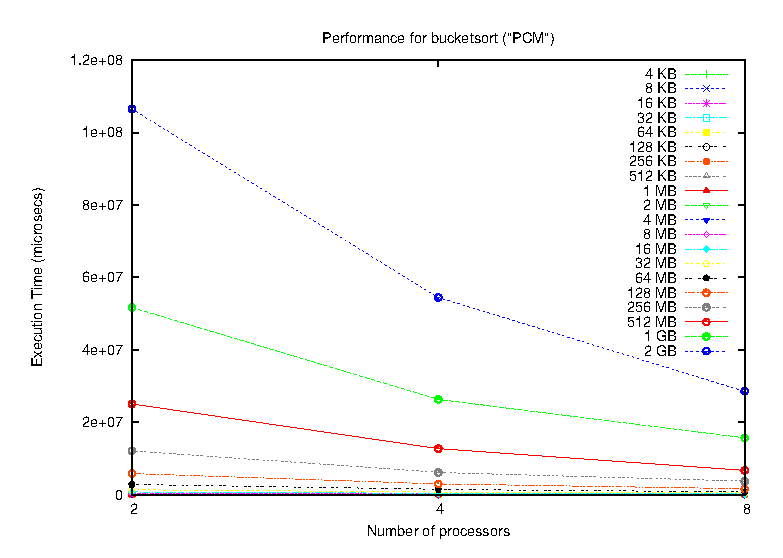
\includegraphics[width=0.4\textwidth]{plots/test_00_PCM/NxTxM/bucketsort_PCM_NxTxM}} 
  	\hspace*{20pt}
  	\subfloat[Samplesort.]{\label{PCM-NxTxM-samplesort}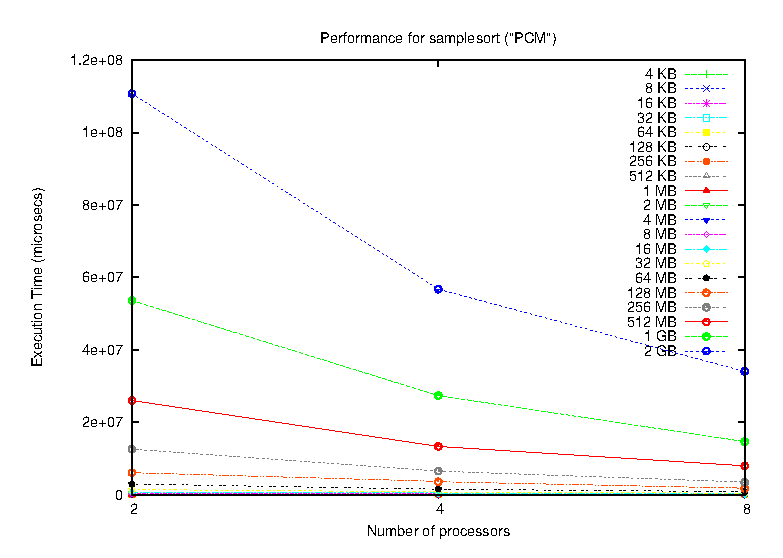
\includegraphics[width=0.4\textwidth]{plots/test_00_PCM/NxTxM/samplesort_PCM_NxTxM}} 
	
	\centering
  	\subfloat[Mergesort.]{\label{PCM-NxTxM-mergesort}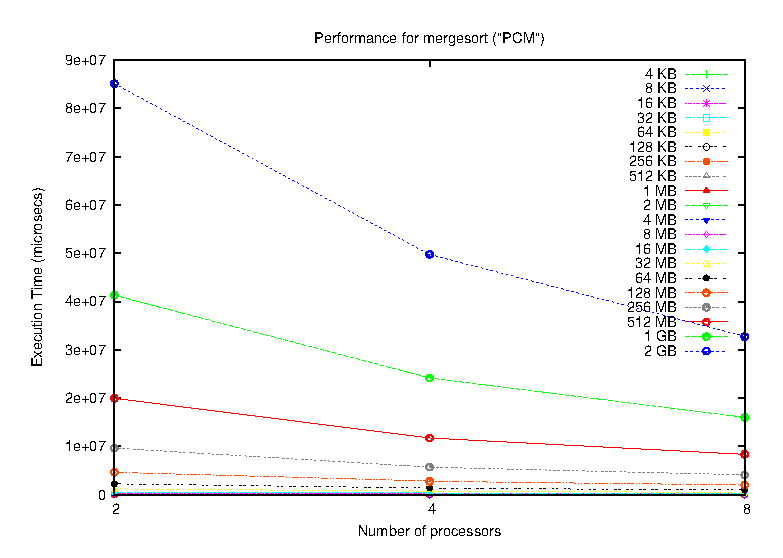
\includegraphics[width=0.4\textwidth]{plots/test_00_PCM/NxTxM/mergesort_PCM_NxTxM}}   
  	\hspace*{20pt}  
  	\subfloat[4-Way Mergesort.]{\label{PCM-NxTxM-kmerge}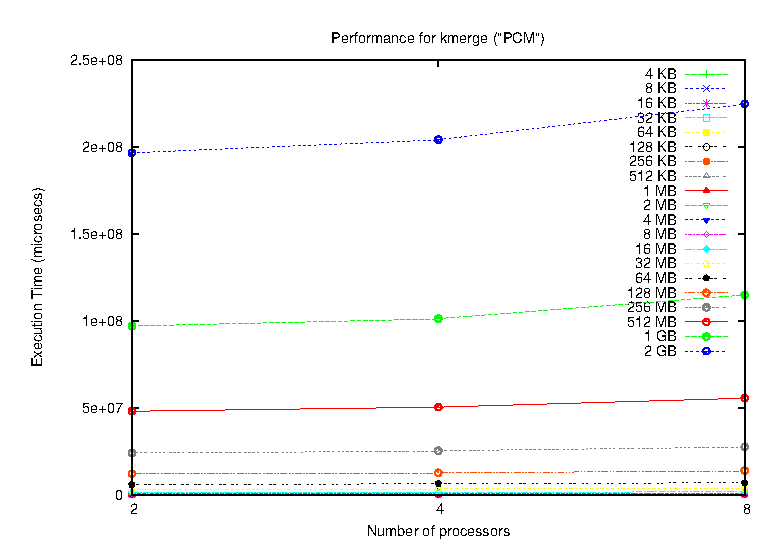
\includegraphics[width=0.4\textwidth]{plots/test_00_PCM/NxTxM/kmerge_PCM_NxTxM}} 
	
	\centering
  	\subfloat[Load-Balanced Mergesort.]{\label{PCM-NxTxM-lbmergesort}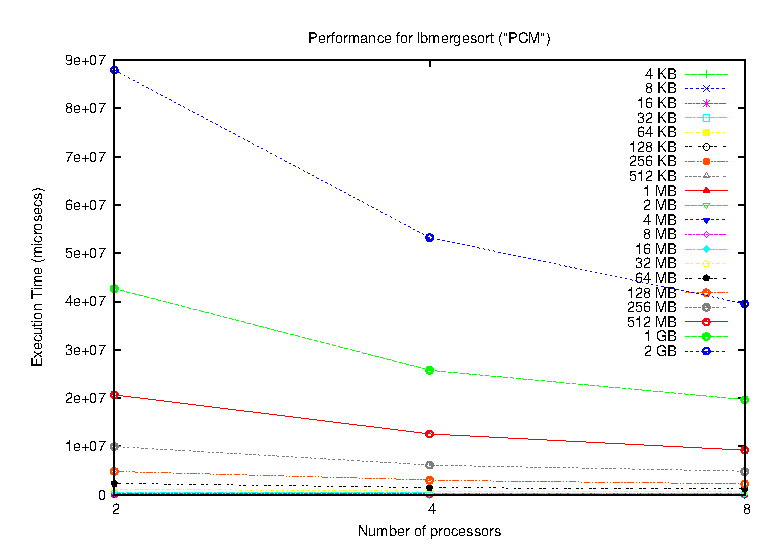
\includegraphics[width=0.4\textwidth]{plots/test_00_PCM/NxTxM/lbmergesort_PCM_NxTxM}} 
  	\hspace*{20pt}  
  	\subfloat[Load-Balanced Multi-Way Mergesort.]{\label{PCM-NxTxM-lbkmergesort}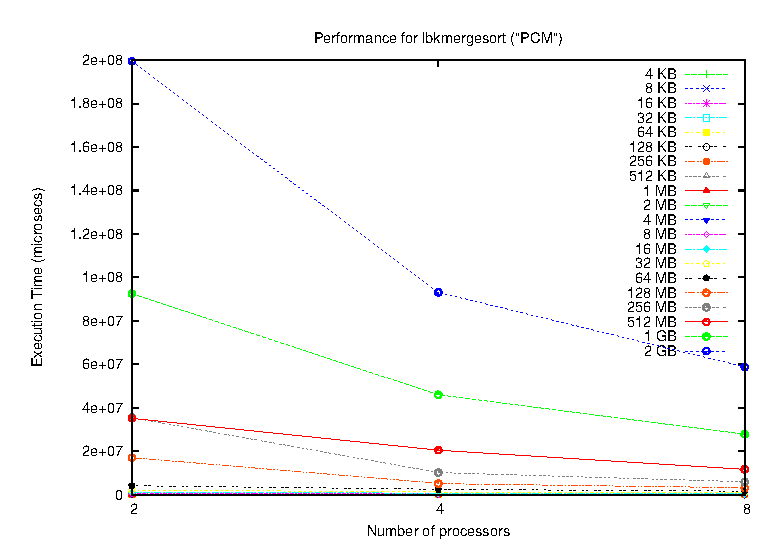
\includegraphics[width=0.4\textwidth]{plots/test_00_PCM/NxTxM/lbkmergesort_PCM_NxTxM}} 	
  	
	\caption{\textit{Intel Xeon X5670}. Time Completion of Sorting Algorithms by varying the parallelism degree. Each shape on a graphic represents the Time Completion of a certain Sorting Algorithm for a data set of specific size.}
	\label{PCM-NxTxM}
\end{figure}
 
\begin{figure}[!ht]
	\centering
	\subfloat[Quicksort.]{\label{PCM-MxTxN-sequential}\includegraphics[width=0.4\textwidth]{plots/test_00_PCM/MxTxN/quicksort_PCM_MxTxN}} 
	\hspace*{20pt}	
  	\subfloat[Bitonicsort.]{\label{PCM-MxTxN-bitonicsort}\includegraphics[width=0.4\textwidth]{plots/test_00_PCM/MxTxN/bitonicsort_PCM_MxTxN}} 
  		
	\centering
	\subfloat[Bucketsort.]{\label{PCM-MxTxN-bucketsort}\includegraphics[width=0.4\textwidth]{plots/test_00_PCM/MxTxN/bucketsort_PCM_MxTxN}} 
  	\hspace*{20pt}
  	\subfloat[Samplesort.]{\label{PCM-MxTxN-samplesort}\includegraphics[width=0.4\textwidth]{plots/test_00_PCM/MxTxN/samplesort_PCM_MxTxN}} 
	
	\centering
  	\subfloat[Mergesort.]{\label{PCM-MxTxN-mergesort}\includegraphics[width=0.4\textwidth]{plots/test_00_PCM/MxTxN/mergesort_PCM_MxTxN}}   
  	\hspace*{20pt}  
  	\subfloat[4-Way Mergesort.]{\label{PCM-MxTxN-kmerge}\includegraphics[width=0.4\textwidth]{plots/test_00_PCM/MxTxN/kmerge_PCM_MxTxN}} 
	
	\centering
  	\subfloat[Load-Balanced Mergesort.]{\label{PCM-MxTxN-lbmergesort}\includegraphics[width=0.4\textwidth]{plots/test_00_PCM/MxTxN/lbmergesort_PCM_MxTxN}} 
  	\hspace*{20pt}  
  	\subfloat[Load-Balanced Multi-Way Mergesort.]{\label{PCM-MxTxN-lbkmergesort}\includegraphics[width=0.4\textwidth]{plots/test_00_PCM/MxTxN/lbkmergesort_PCM_MxTxN}} 
  	
	\caption{\textit{Intel Xeon X5670}. Time Completion of Sorting Algorithms for increasing sizes of the data set. }
	\label{PCM-MxTxN}
\end{figure} 


\paragraph{Comparison between Sorting Algorithms} Figures~\ref{PCM-NxTxA-small} and~\ref{PCM-NxTxA-large} highlight the behaviour of different Sorting Algorithms for specifics sizes of the data set. Notice an interesting aspect reguarding \textbf{small} data sets: we have seen that on $Pianosa$ best algorithms were \textit{qsort} and parallel \textit{Mergesort} (at low parallelism degrees). On this architecture things are deeply different and this is likely due to the fact that processes communications now take place in shared memory. Figure~\ref{PCM-NxTxA-small} shows that most of Sorting Algorithms, altough still far away from the linear scalability, definitely outperform \textit{qsort} (at least for sizes of the data set greater than 8 KB). Moreover, \textit{Mergesort} confirms itself as one of the best Sorting Algorithms both for small data sets and now even for \textbf{large} data sets, together with \textit{Bitonicsort}, \textit{Bucketsort}, \textit{Samplesort} and \textit{Load-Balanced (Multi-Way) Mergesort}.

\begin{figure}[!ht]
	\centering
	\subfloat[Data set of 1K integers.]{\label{PCM-NxTxA-1M}\includegraphics[width=0.4\textwidth]{plots/test_00_PCM/NxTxA/M1024_PCM_NxTxA}} 
	\hspace*{20pt}	
  	\subfloat[Data set of 2K integers.]{\label{PCM-NxTxA-2M}\includegraphics[width=0.4\textwidth]{plots/test_00_PCM/NxTxA/M2048_PCM_NxTxA}} 
  		
	\centering
	\subfloat[Data set of 4K integers.]{\label{PCM-NxTxA-4M}\includegraphics[width=0.4\textwidth]{plots/test_00_PCM/NxTxA/M4096_PCM_NxTxA}} 
  	\hspace*{20pt}
  	\subfloat[Data set of 8K integers.]{\label{PCM-NxTxA-8M}\includegraphics[width=0.4\textwidth]{plots/test_00_PCM/NxTxA/M8192_PCM_NxTxA}} 
	
	\centering
  	\subfloat[Data set of 16K integers.]{\label{PCM-NxTxA-16M}\includegraphics[width=0.4\textwidth]{plots/test_00_PCM/NxTxA/M16384_PCM_NxTxA}}   
  	\hspace*{20pt}  
  	\subfloat[Data set of 32K integers.]{\label{PCM-NxTxA-32M}\includegraphics[width=0.4\textwidth]{plots/test_00_PCM/NxTxA/M32768_PCM_NxTxA}} 
  	
	\centering
  	\subfloat[Data set of 64K integers.]{\label{PCM-NxTxA-16M}\includegraphics[width=0.4\textwidth]{plots/test_00_PCM/NxTxA/M65536_PCM_NxTxA}}   
  	\hspace*{20pt}  
  	\subfloat[Data set of 128K integers.]{\label{PCM-NxTxA-32M}\includegraphics[width=0.4\textwidth]{plots/test_00_PCM/NxTxA/M131072_PCM_NxTxA}}   	
  	
	%\caption{\textit{Intel Xeon X5670}. Time Completion for sorting \textit{small} data sets. Each graphic represents a data set of fixed size, while each shape on a graphic shows the Time Completion of a certain Sorting Algorithm for that data set.}
	%\label{PCM-NxTxA-small}
\end{figure} 

\begin{figure}[!ht]
	\ContinuedFloat
	\centering
	\subfloat[Data set of 256K integers.]{\label{PCM-NxTxA-1M}\includegraphics[width=0.4\textwidth]{plots/test_00_PCM/NxTxA/M262144_PCM_NxTxA}} 
	\hspace*{20pt}	
  	\subfloat[Data set of 512K integers.]{\label{PCM-NxTxA-2M}\includegraphics[width=0.4\textwidth]{plots/test_00_PCM/NxTxA/M524288_PCM_NxTxA}} 

	\centering
	\subfloat[Data set of 1M integers.]{\label{PCM-NxTxA-1M}\includegraphics[width=0.4\textwidth]{plots/test_00_PCM/NxTxA/M1048576_PCM_NxTxA}} 
	\hspace*{20pt}	
  	\subfloat[Data set of 2M integers.]{\label{PCM-NxTxA-2M}\includegraphics[width=0.4\textwidth]{plots/test_00_PCM/NxTxA/M2097152_PCM_NxTxA}} 
  		
	\centering
	\subfloat[Data set of 4M integers.]{\label{PCM-NxTxA-4M}\includegraphics[width=0.4\textwidth]{plots/test_00_PCM/NxTxA/M4194304_PCM_NxTxA}} 
  	\hspace*{20pt}
  	\subfloat[Data set of 8M integers.]{\label{PCM-NxTxA-8M}\includegraphics[width=0.4\textwidth]{plots/test_00_PCM/NxTxA/M8388608_PCM_NxTxA}} 
	
	\centering
  	\subfloat[Data set of 16M integers.]{\label{PCM-NxTxA-16M}\includegraphics[width=0.4\textwidth]{plots/test_00_PCM/NxTxA/M16777216_PCM_NxTxA}}   
  	\hspace*{20pt}  
  	\subfloat[Data set of 32M integers.]{\label{PCM-NxTxA-32M}\includegraphics[width=0.4\textwidth]{plots/test_00_PCM/NxTxA/M33554432_PCM_NxTxA}} 
  	
	\caption{\textit{Intel Xeon X5670}. Time Completion for sorting \textit{small} data sets. Each graphic represents a data set of fixed size, while each shape on a graphic shows the Time Completion of a certain Sorting Algorithm for that data set.}
	\label{PCM-NxTxA-small}
\end{figure} 

\begin{figure}[!ht]
	\centering
	\subfloat[Data set of 64M integers.]{\label{PCM-NxTxA-64M}\includegraphics[width=0.4\textwidth]{plots/test_00_PCM/NxTxA/M67108864_PCM_NxTxA}} 
	\hspace*{20pt}	
  	\subfloat[Data set of 128M integers.]{\label{PCM-NxTxA-128M}\includegraphics[width=0.4\textwidth]{plots/test_00_PCM/NxTxA/M134217728_PCM_NxTxA}} 
  		
	\centering
	\subfloat[Data set of 256M integers.]{\label{PCM-NxTxA-256M}\includegraphics[width=0.4\textwidth]{plots/test_00_PCM/NxTxA/M268435456_PCM_NxTxA}} 
  	\hspace*{20pt}
  	\subfloat[Data set of 512M integers.]{\label{PCM-NxTxA-512M}\includegraphics[width=0.4\textwidth]{plots/test_00_PCM/NxTxA/M536870912_PCM_NxTxA}} 
	
	\caption{\textit{Intel Xeon X5670}. Time Completion for sorting \textit{large} data sets. Each graphic represents a data set of fixed size, while each shape on a graphic shows the Time Completion of a certain Sorting Algorithm for that data set.}
	\label{PCM-NxTxA-large}
\end{figure} 

\begin{figure}[!ht]
	\centering
	\subfloat[Parallelism degree 2.]{\label{PCM-MxTxA-n2}\includegraphics[width=0.5\textwidth]{plots/test_00_PCM/MxTxA/n2_PCM_MxTxA}} 
	
	\centering
  	\subfloat[Parallelism degree 4.]{\label{PCM-MxTxA-n4}\includegraphics[width=0.5\textwidth]{plots/test_00_PCM/MxTxA/n4_PCM_MxTxA}} 
  		
	\centering
	\subfloat[Parallelism degree 8.]{\label{PCM-MxTxA-n8}\includegraphics[width=0.5\textwidth]{plots/test_00_PCM/MxTxA/n8_PCM_MxTxA}} 
  	
	\caption{\textit{Intel Xeon X5670}. Time Completion for sorting data sets with fixed parallelism degree.}
	\label{PCM-MxTxA}
\end{figure}

\clearpage

\subsubsection{PCM}
$PCM$ is a cluster of shared memory machines, thus all considerations reguarding mapping of processes to cores made in~\ref{fram-intr} become matter of study. Even the official guide of \textit{mvapich2}, the version of MPI that we have used to exploit Infiniband, emphasizes the importance of process-to-core mapping: as shown in~\cite{MVAPICH2-MAPPING}, different allocations of processes to cores can have a significant impact on the cost of communications. In principle, an entire study could be dedicated to this topic, leading to a lot of possible mappings, each one based on its reasonable heuristic. Obviously, we had to limit our analysis to a subset of the most simple mappings. In particular, we have studied the following configurations:   
\begin{itemize}
\item \textbf{Sequential mapping}. Adjacent ranks mapped on adjacent \textit{cores}. E.g., given two CPUs each one with 4 cores and 8 MPI processes, rank 0 goes on the first core of the \textit{first} CPU, rank 1 goes on the second core of the \textit{first} CPU, ..., rank 5 goes on the first core of the \textit{second} CPU and so on.
\item \textbf{Interleaved mapping}. Adjacent ranks mapped on adjacent \textit{CPUs}. E.g., given two CPUs each one with 4 cores and 8 MPI processes, rank 0 goes on the first core of the \textit{first} CPU, rank 1 goes on the first core of the \textit{second} CPU, rank 2 goes on the second core of the \textit{first} CPU and so on.
\item \textbf{Algorithm-specific mapping}. We have also studied a few mapping based on the nature of a specific Sorting Algorithm, like \textit{Mergesort} and \textit{Quicksort}. For instance, a mapping could be designed to let the most critical part of a stencil to take place in shared memory rather than inter-node.  
\end{itemize}
In the following, we will consider only the \textit{sequential mapping} because we have practically experienced that collective communications (in particular, the \textit{gather}) are more cost-effective than for other mappings. For more informations about the results obtained with other mappings the reader could refer to specific material attached to this report.


\paragraph{Scalability of Sorting Algorithms}

\paragraph{Comparison between Sorting Algorithms}

\clearpage


\subsection{Comparing the results}

\section{What we are going to do}
In this report we explained goals and current state of our work. First, we spent a lot of efforts in understanding the state of the art of parallel sorting by searching in books and papers. Once gathered sufficient informations, we designed a framework to address all the problems that would have been common to all our algorithms: e.g.: generation, loading and storing of datas, timing, initialization of the MPI environment and so on. Keep in mind that, thanks to its modularity, we will be able to exploit the features of our framework for any new sorting algorithm we would like to implement. 

We have already implemented and tested all the algorithms we described. We have performed some tests on Pianosa, the cluster at our department, both to check the correct behaviour of the algorithms and to start analyzing the performance. Some of the algorithms still needs some minor fixes for what concerns the implementation.

What are going to do in the next weeks:
\begin{itemize}
\item ultimating the implementation of the framework to handle huge data sets;
\item refining the implementation of the algorithms in order to fix some little bugs;
\item performing the same tests we run on pianosa on the ''Physics' cluster'';
\item analyzing both the scalability and the algorithm-efficieny of our algorithms;
\item checking (and understanding) for potential mismatches between the scalability obtained on Pianosa and the one on the ''Physics' cluster'';
\item writing a final version of this report.
\end{itemize}


                                                                    

%\lstinputlisting{mapreduce_types.code}

%\begin{figure}
%        \centerline{
%               \mbox{\includegraphics[scale=0.88]{CompletionTime_64}}
%        }
%        \caption{The completion time for the benchmark using a matrix of 64MB.}
%        \label{CompletionTime64}
%\end{figure}


\pagebreak

\begin{thebibliography}{13}
\bibitem{FERR}{Paolo Ferragina. \textit{The magic of Algorithms!.} Lectures notes in Algorithm Engineering, 2010}
\bibitem{CPSA}{Nancy M. Amato	 and Ravishankar Iyer and Sharad Sundaresan and Yan Wu.\textit{A Comparison of Parallel Sorting Algorithms on Different Architectures.} Technical Report 98-029, Department of Computer Science, Texas A$\&$M University, January 1996. }
\bibitem{CSPA2}{Marc Moreno Maza . \textit{CS855: Parallel Sorting Algorithms.} Technical Report, Department of Computer Science, The University of Western Ontario, February 2008.}
\bibitem{NPSA}{David R. Cheng and Alan Edelman and John R. Gilbert and Viral Shah. \textit{A Novel Parallel Sorting Algorithm for Contemporary Architectures.} In ALENEX06, May 2007.}
\end{thebibliography}
\end{document}
